%% LyX 2.3.7 created this file.  For more info, see http://www.lyx.org/.
%% Do not edit unless you really know what you are doing.
\documentclass[journal,article,submit,pdftex,moreauthors]{Definitions/mdpi}
\usepackage[T1]{fontenc}
\usepackage[utf8]{inputenc}
\usepackage{array}
\usepackage{float}
\usepackage{booktabs}
\usepackage{url}
\usepackage{amstext}
\usepackage{graphicx}

\makeatletter

%%%%%%%%%%%%%%%%%%%%%%%%%%%%%% LyX specific LaTeX commands.

\Title{Combining Parallel Stochastic Methods and Mixed Termination Rules
in Optimization}

\TitleCitation{Combining Parallel Stochastic Methods and Mixed Termination Rules
in Optimization}

\Author{Vasileios Charilogis$^{1}$, Ioannis G. Tsoulos$^{2,*}$, Anna Maria
Gianni$^{3}$}

\AuthorNames{V. Charilogis, I.G. Tsoulos, A.M. Gianni}

\AuthorCitation{Charilogis V.; Tsoulos I.G.; Gianni A.M; }


\address{$^{1}$\quad{}Department of Informatics and Telecommunications,
University of Ioannina, Greece; v.charilog@uoi.gr\\
$^{2}$\quad{}Department of Informatics and Telecommunications, University
of Ioannina, Greece; itsoulos@uoi.gr\\
$^{3}$\quad{}Department of Informatics and Telecommunications, University
of Ioannina, Greece; am.gianni@uoi.gr}


\corres{Correspondence: itsoulos@uoi.gr;}


\firstnote{Current address: Department of Informatics and Telecommunications,
University of Ioannina, Greece.}


\secondnote{These authors contributed equally to this work.}


\abstract{Parallel optimization enables faster and more efficient problem-solving
by reducing computational resource consumption and time. By simultaneously
combining multiple methods, such as evolutionary algorithms and swarm-based
optimization, effective exploration of the search space and achievement
of optimal solutions in shorter time frames are realized. In this
study, a combination of termination criteria is proposed, utilizing
three different criteria to end the algorithmic process. These criteria
include measuring the difference between optimal values in successive
iterations, calculating the mean value of the cost function in each
iteration, and the so-called \textquotedbl DoubleBox\textquotedbl{}
criterion, which is based on the relative variance of the best value
of the objective cost function over a specific number of iterations.
The problem is addressed through the parallel execution of three different
optimization methods (PSO, Differential Evolution, Multistart). Each
method operates independently on separate computational units with
the goal of faster discovery of the optimal solution and more efficient
use of computational resources. The optimal solution identified in
each iteration is transferred to the other computational units. The
proposed enhancements were tested on a series of well-known optimization
problems from relevant literature, demonstrating significant improvements
in convergence speed and solution quality compared to traditional
approaches.}


\keyword{Global optimization; Parallel techniques; Termination rules; Evolutionary
techniques}

\newcommand*\LyXZeroWidthSpace{\hspace{0pt}}
%% Because html converters don't know tabularnewline
\providecommand{\tabularnewline}{\\}
\floatstyle{ruled}
\newfloat{algorithm}{tbp}{loa}
\providecommand{\algorithmname}{Algorithm}
\floatname{algorithm}{\protect\algorithmname}

%%%%%%%%%%%%%%%%%%%%%%%%%%%%%% User specified LaTeX commands.
%  LaTeX support: latex@mdpi.com 
%  For support, please attach all files needed for compiling as well as the log file, and specify your operating system, LaTeX version, and LaTeX editor.

%=================================================================


% For posting an early version of this manuscript as a preprint, you may use "preprints" as the journal and change "submit" to "accept". The document class line would be, e.g., \documentclass[preprints,article,accept,moreauthors,pdftex]{mdpi}. This is especially recommended for submission to arXiv, where line numbers should be removed before posting. For preprints.org, the editorial staff will make this change immediately prior to posting.

%--------------------
% Class Options:
%--------------------
%----------
% journal
%----------
% Choose between the following MDPI journals:
% acoustics, actuators, addictions, admsci, adolescents, aerospace, agriculture, agriengineering, agronomy, ai, algorithms, allergies, alloys, analytica, animals, antibiotics, antibodies, antioxidants, applbiosci, appliedchem, appliedmath, applmech, applmicrobiol, applnano, applsci, aquacj, architecture, arts, asc, asi, astronomy, atmosphere, atoms, audiolres, automation, axioms, bacteria, batteries, bdcc, behavsci, beverages, biochem, bioengineering, biologics, biology, biomass, biomechanics, biomed, biomedicines, biomedinformatics, biomimetics, biomolecules, biophysica, biosensors, biotech, birds, bloods, blsf, brainsci, breath, buildings, businesses, cancers, carbon, cardiogenetics, catalysts, cells, ceramics, challenges, chemengineering, chemistry, chemosensors, chemproc, children, chips, cimb, civileng, cleantechnol, climate, clinpract, clockssleep, cmd, coasts, coatings, colloids, colorants, commodities, compounds, computation, computers, condensedmatter, conservation, constrmater, cosmetics, covid, crops, cryptography, crystals, csmf, ctn, curroncol, currophthalmol, cyber, dairy, data, dentistry, dermato, dermatopathology, designs, diabetology, diagnostics, dietetics, digital, disabilities, diseases, diversity, dna, drones, dynamics, earth, ebj, ecologies, econometrics, economies, education, ejihpe, electricity, electrochem, electronicmat, electronics, encyclopedia, endocrines, energies, eng, engproc, ent, entomology, entropy, environments, environsciproc, epidemiologia, epigenomes, est, fermentation, fibers, fintech, fire, fishes, fluids, foods, forecasting, forensicsci, forests, foundations, fractalfract, fuels, futureinternet, futureparasites, futurepharmacol, futurephys, futuretransp, galaxies, games, gases, gastroent, gastrointestdisord, gels, genealogy, genes, geographies, geohazards, geomatics, geosciences, geotechnics, geriatrics, hazardousmatters, healthcare, hearts, hemato, heritage, highthroughput, histories, horticulturae, humanities, humans, hydrobiology, hydrogen, hydrology, hygiene, idr, ijerph, ijfs, ijgi, ijms, ijns, ijtm, ijtpp, immuno, informatics, information, infrastructures, inorganics, insects, instruments, inventions, iot, j, jal, jcdd, jcm, jcp, jcs, jdb, jeta, jfb, jfmk, jimaging, jintelligence, jlpea, jmmp, jmp, jmse, jne, jnt, jof, joitmc, jor, journalmedia, jox, jpm, jrfm, jsan, jtaer, jzbg, kidney, kidneydial, knowledge, land, languages, laws, life, liquids, literature, livers, logics, logistics, lubricants, lymphatics, machines, macromol, magnetism, magnetochemistry, make, marinedrugs, materials, materproc, mathematics, mca, measurements, medicina, medicines, medsci, membranes, merits, metabolites, metals, meteorology, methane, metrology, micro, microarrays, microbiolres, micromachines, microorganisms, microplastics, minerals, mining, modelling, molbank, molecules, mps, msf, mti, muscles, nanoenergyadv, nanomanufacturing, nanomaterials, ncrna, network, neuroglia, neurolint, neurosci, nitrogen, notspecified, nri, nursrep, nutraceuticals, nutrients, obesities, oceans, ohbm, onco, oncopathology, optics, oral, organics, organoids, osteology, oxygen, parasites, parasitologia, particles, pathogens, pathophysiology, pediatrrep, pharmaceuticals, pharmaceutics, pharmacoepidemiology, pharmacy, philosophies, photochem, photonics, phycology, physchem, physics, physiologia, plants, plasma, pollutants, polymers, polysaccharides, poultry, powders, preprints, proceedings, processes, prosthesis, proteomes, psf, psych, psychiatryint, psychoactives, publications, quantumrep, quaternary, qubs, radiation, reactions, recycling, regeneration, religions, remotesensing, reports, reprodmed, resources, rheumato, risks, robotics, ruminants, safety, sci, scipharm, seeds, sensors, separations, sexes, signals, sinusitis, skins, smartcities, sna, societies, socsci, software, soilsystems, solar, solids, sports, standards, stats, stresses, surfaces, surgeries, suschem, sustainability, symmetry, synbio, systems, taxonomy, technologies, telecom, test, textiles, thalassrep, thermo, tomography, tourismhosp, toxics, toxins, transplantology, transportation, traumacare, traumas, tropicalmed, universe, urbansci, uro, vaccines, vehicles, venereology, vetsci, vibration, viruses, vision, waste, water, wem, wevj, wind, women, world, youth, zoonoticdis 

%---------
% article
%---------
% The default type of manuscript is "article", but can be replaced by: 
% abstract, addendum, article, book, bookreview, briefreport, casereport, comment, commentary, communication, conferenceproceedings, correction, conferencereport, entry, expressionofconcern, extendedabstract, datadescriptor, editorial, essay, erratum, hypothesis, interestingimage, obituary, opinion, projectreport, reply, retraction, review, perspective, protocol, shortnote, studyprotocol, systematicreview, supfile, technicalnote, viewpoint, guidelines, registeredreport, tutorial
% supfile = supplementary materials

%----------
% submit
%----------
% The class option "submit" will be changed to "accept" by the Editorial Office when the paper is accepted. This will only make changes to the frontpage (e.g., the logo of the journal will get visible), the headings, and the copyright information. Also, line numbering will be removed. Journal info and pagination for accepted papers will also be assigned by the Editorial Office.

%------------------
% moreauthors
%------------------
% If there is only one author the class option oneauthor should be used. Otherwise use the class option moreauthors.

%---------
% pdftex
%---------
% The option pdftex is for use with pdfLaTeX. If eps figures are used, remove the option pdftex and use LaTeX and dvi2pdf.

%=================================================================
% MDPI internal commands - do not modify
\firstpage{1} 
 
\setcounter{page}{\@firstpage} 

\pubvolume{1}
\issuenum{1}
\articlenumber{0}
\pubyear{2023}
\copyrightyear{2023}
%\externaleditor{Academic Editor: Firstname Lastname} % For journal Automation, please change Academic Editor to "Communicated by"
\datereceived{}
\daterevised{ } % Comment out if no revised date
\dateaccepted{}
\datepublished{}
%\datecorrected{} % Corrected papers include a "Corrected: XXX" date in the original paper.
%\dateretracted{} % Corrected papers include a "Retracted: XXX" date in the original paper.
\hreflink{https://doi.org/} % If needed use \linebreak
%\doinum{}
%------------------------------------------------------------------
% The following line should be uncommented if the LaTeX file is uploaded to arXiv.org
%\pdfoutput=1

%=================================================================
% Add packages and commands here. The following packages are loaded in our class file: fontenc, inputenc, calc, indentfirst, fancyhdr, graphicx, epstopdf, lastpage, ifthen, lineno, float, amsmath, setspace, enumitem, mathpazo, booktabs, titlesec, etoolbox, tabto, xcolor, soul, multirow, microtype, tikz, totcount, changepage, attrib, upgreek, cleveref, amsthm, hyphenat, natbib, hyperref, footmisc, url, geometry, newfloat, caption

%=================================================================
%% Please use the following mathematics environments: Theorem, Lemma, Corollary, Proposition, Characterization, Property, Problem, Example, ExamplesandDefinitions, Hypothesis, Remark, Definition, Notation, Assumption
%% For proofs, please use the proof environment (the amsthm package is loaded by the MDPI class).

%=================================================================
% The fields PACS, MSC, and JEL may be left empty or commented out if not applicable
%\PACS{J0101}
%\MSC{}
%\JEL{}

%%%%%%%%%%%%%%%%%%%%%%%%%%%%%%%%%%%%%%%%%%
% Only for the journal Diversity
%\LSID{\url{http://}}

%%%%%%%%%%%%%%%%%%%%%%%%%%%%%%%%%%%%%%%%%%
% Only for the journal Applied Sciences:
%\featuredapplication{Authors are encouraged to provide a concise description of the specific application or a potential application of the work. This section is not mandatory.}
%%%%%%%%%%%%%%%%%%%%%%%%%%%%%%%%%%%%%%%%%%

%%%%%%%%%%%%%%%%%%%%%%%%%%%%%%%%%%%%%%%%%%
% Only for the journal Data:
%\dataset{DOI number or link to the deposited data set in cases where the data set is published or set to be published separately. If the data set is submitted and will be published as a supplement to this paper in the journal Data, this field will be filled by the editors of the journal. In this case, please make sure to submit the data set as a supplement when entering your manuscript into our manuscript editorial system.}

%\datasetlicense{license under which the data set is made available (CC0, CC-BY, CC-BY-SA, CC-BY-NC, etc.)}

%%%%%%%%%%%%%%%%%%%%%%%%%%%%%%%%%%%%%%%%%%
% Only for the journal Toxins
%\keycontribution{The breakthroughs or highlights of the manuscript. Authors can write one or two sentences to describe the most important part of the paper.}

%%%%%%%%%%%%%%%%%%%%%%%%%%%%%%%%%%%%%%%%%%
% Only for the journal Encyclopedia
%\encyclopediadef{Instead of the abstract}
%\entrylink{The Link to this entry published on the encyclopedia platform.}
%%%%%%%%%%%%%%%%%%%%%%%%%%%%%%%%%%%%%%%%%%

%%%%%%%%%%%%%%%%%%%%%%%%%%%%%%%%%%%%%%%%%%
% Only for the journal Advances in Respiratory Medicine
%\addhighlights{yes}
%\renewcommand{\addhighlights}{%

%\noindent This is an obligatory section in “Advances in Respiratory Medicine”, whose goal is to increase the discoverability and readability of the article via search engines and other scholars. Highlights should not be a copy of the abstract, but a simple text allowing the reader to quickly and simplified find out what the article is about and what can be cited from it. Each of these parts should be devoted up to 2~bullet points.\vspace{3pt}\\
%\textbf{What are the main findings?}
% \begin{itemize}[labelsep=2.5mm,topsep=-3pt]
% \item First bullet.
% \item Second bullet.
% \end{itemize}\vspace{3pt}
%\textbf{What is the implication of the main finding?}
% \begin{itemize}[labelsep=2.5mm,topsep=-3pt]
% \item First bullet.
% \item Second bullet.
% \end{itemize}
%}
%%%%%%%%%%%%%%%%%%%%%%%%%%%%%%%%%%%%%%%%%%

\makeatother

\begin{document}
\maketitle

\section{Introduction}

The problem of finding the global minimum of a multidimensional function
occurs in various scientific areas and has wide applications. In this
the programmer seeks the absolute minimum of a function subject to
some assumptions or constraints. The objective function is defined
as $f:S\rightarrow R,S\subset R^{n}$ and the mathematical formulation
of the global optimization problem is as follows:
\begin{equation}
x^{*}=\mbox{arg}\min_{x\in S}f(x).\label{eq:eq1-1}
\end{equation}
where the set $S$ is as follows: \textbf{
\[
S=\left[a_{1},b_{1}\right]\otimes\left[a_{2},b_{2}\right]\otimes\ldots\left[a_{n},b_{n}\right]
\]
}Such problems frequently arise in sciences like physics, where genetic
algorithms prove effective in locating positions in magnetic plasmas
and in developing optimization tools \citep{go_physics1}. Additionally,
the combined use of various optimization techniques enhances performance
and stability in complex problems \citep{go_physics2}. Furthermore,
the hybrid approach that combines artificial physics techniques with
particle swarm optimization has proven to be particularly effective
in solving energy allocation problems \citep{go_physics3}. In the
field of chemistry, minimizing potential energy functions is crucial
for understanding the ground states of molecular clusters and proteins
\citep{go_chemistry1}. Optimizing these functions has been used for
accurate protein structure prediction, with results closely matching
crystal structures \citep{go_chemistry2}. Moreover, a new computational
framework combining variance-based methods with artificial neural
networks has significantly improved accuracy and reduced computational
cost in sensitivity analysis \citep{go_chemistry3}. Even in the field
of economics, optimization plays a crucial role. The particle swarm
optimization (PSO) method is shown to be highly effective in solving
the economic dispatch problem in power systems, providing higher quality
solutions with greater efficiency compared to genetic algorithms \citep{go_econ1}.
Additionally, a multi-objective optimization approach for economic
load dispatch and emission reduction in hydroelectric and thermal
plants achieves optimal solutions that align with the user's preferences
and goals \citep{go_econ2}. Finally, optimization is also applied
in biological process models \citep{go_med1} and medical data classification,
achieving high accuracy in diagnosing diseases and analyzing genomes
\citep{go_med2}. A series of methods have been proposed in the recent
literature to handle problems of Equation \ref{eq:eq1-1}. Methods
used to handle problems of Equation \ref{eq:eq1-1} are usually divided
into two categories:\textbf{ }deterministic and stochastic methods.
In the first category, the most common method is the interval method
\citep{interval1,interval2}, where the set $S$ is divided through
a series of steps into subregions and some subregions that do not
contain the global solution can be removed using some pre-defined
criteria. The second category contains stochastic techniques that
do not guarantee finding the total minimum, they are easier to program
since they do not rely on some assumptions about the objective function.
In addition, they also constitute the vast majority of global optimization
methods. Among them, there are methods based on considerations derived
from Physics, such as the Simulated Annealing method\citep{Kirkpatrick},
the Henry's Gas Solubility Optimization (HGSO) \citep{Hashim}, the
Gravitational Search Algorithm (GSA) \citep{Rashedi}, the Small World
Optimization Algorithm (SWOA) \citep{Du-Wu}, etc. Also, a series
of evolutionary based techniques have also been suggested for Global
Optimization problems, such as Genetic Algorithms \citep{Goldberg},
the Differential Evolution method \citep{Das,Charilogis}, Particle
Swarm Optimization (PSO) \citep{Kennedy,Charilogis2}, Ant Colony
Optimization (ACO) \citep{Dorigo}, Bat Algorithm (BA) \citep{Yang},
Whale Optimization Algorithm (WOA) \citep{Mirjalili}, Grasshopper
Optimization Algorithm (GOA) \citep{Saremi}, etc.

However, the above optimization methods require significant computational
power and time. Therefore, parallel processing of these methods is
essential. Recently, various methods have been proposed to leverage
parallel processing. Specifically, one study details the parallel
implementation of the Particle Swarm Optimization (PSO) algorithm,
which improves performance for load-balanced problems but shows reduced
efficiency for load-imbalanced ones. The study suggests using larger
particle populations and implementing asynchronous processing to enhance
performance \citep{parallel-pso}. Another review provides a comprehensive
overview of derivative-free optimization methods, useful for problems
where objective and constraint functions come only from a black-box
or simulator interface. The review focuses on recent developments
and categorizes methods based on assumptions about functions and their
characteristics \citep{parallel-multistart}. Lastly, the PDoublePop
software is presented, which implements parallel genetic algorithms
with advanced features, such as an enhanced stopping rule and advanced
mutation schemes. The software allows for coding the objective function
in C++ or Fortran77 and has been tested on well-known benchmark functions,
showing promising results \citep{parallel-doublepop}. Moreover, there
are methods that utilize GPU architectures for solving complex optimization
problems. In the case of the Traveling Salesman Problem (TSP), a parallel
GPU implementation has been developed to achieve high performance
on large scales, solving problems up to 6,000 cities with great efficiency
\citep{msgpu1}. Additionally, the use of the multi-start model in
local search algorithms has proven to be particularly effective when
combined with GPUs, reducing computation time and improving solution
quality for large and time-intensive problems \citep{msgpu2}. Finally,
a parallel algorithm using Peano curves for dimension reduction has
demonstrated significant improvements in speed and efficiency when
run on GPUs, compared to CPU-only implementations, for multidimensional
problems with multiple local minima \citep{msgpu3}. Parallel optimization
represents a significant approach in the field of optimization problem-solving
and is applied across a broad range of applications, including the
optimization of machine learning model parameters. In the case of
GraphLab, a platform is presented that enhances existing abstract
methods, such as MapReduce, for parallel execution of machine learning
algorithms with high performance and accuracy \citep{Low Gon}. Additionally,
the new MARSAOP method for hyperparameter optimization uses multidimensional
spirals as surrogates and dynamic coordinate search to achieve high-quality
solutions with limited computational cost \citep{Yangyang}. Lastly,
the study proposes a processing time estimation system using machine
learning models to adapt to complex distributions and improve production
scheduling, achieving significant reduction in completion time \citep{Yamashiro}.

The use of parallel optimization has brought significant advancements
in solving complex control and design problems \citep{Kim Tsai}.
In one case, the parallel application of the Genetic Algorithm with
a Fair Competitive Strategy (HFCGA) has been used for the design of
an optimized cascade controller for ball and beam systems. This approach
allows for the automation of controller parameter tuning, improving
performance compared to traditional methods, with parallel computations
helping to avoid premature convergence to suboptimal solutions \citep{Oh Jong}.
In another case, the advanced Teaching-Learning-Based Optimization
(TLBO) method has been applied to optimize the design of propulsion
control systems with hydrogen peroxide. This method, which includes
improvements in the teaching and learning phases as well as in the
search process, has proven highly effective in addressing uncertainties
in real-world design problems, enhancing both accuracy and convergence
speed of the optimization process \citep{Fatehi}.

Similarly, parallel optimization has significant applications in energy
and resource management. In the case of pump and cooling system management,
a two-stage method based on an innovative multidimensional optimization
algorithm has been proposed, which reduces overall energy consumption
and discrepancies between pump and cooling system flow rates, achieving
significant improvements in energy efficiency \citep{Cai Yang}. In
energy network management, a coordinated scheduled optimization method
has been proposed, which simultaneously considers various energy sources
and uncertainty conditions. This method, using the Competitive Swarm
Optimization (CSO) algorithm and adjusted based on chaos theory, has
proven 50\% faster than other methods and effective in managing uncertainties
and energy \citep{Yu Shahabi}. In topological optimization, parallel
processing through CPUs and GPUs has drastically improved speed and
energy consumption for complex problems, achieving up to 25 times
faster processing and reducing energy consumption by up to 93\% \citep{Ramirez}.
Lastly, in building energy retrofitting, a multi-objective platform
was used for evaluating and optimizing upgrade strategies, demonstrating
that removing subsidies and providing incentives for energy upgrades
yield promising results \citep{Tavakolan}.

In conclusion, parallel optimization has provided significant solutions
to problems related to sustainable development and enhancing sustainability.
In the field of increasing the resilience of energy systems, the development
of strategies for managing severe risks, such as extreme weather conditions
and supplier disruptions, has been improved through parallel optimization,
enabling safer and more cost-effective energy system operations \citep{Lin}.
In addressing groundwater contamination, the use of parallel optimization
has highlighted the potential for faster and more effective design
of remediation methods, significantly reducing computational budgets
and ensuring better results compared to other methods \citep{Pang}.
Finally, in the field of sustainable production, metaheuristic optimization
algorithms have proven useful for improving production scheduling,
promoting resource efficiency, and reducing environmental impacts,
while contributing to the achievement of sustainable development goals
\citep{Ezugwu}. 

By harnessing multiple computational resources, parallel optimization
allows for the simultaneous execution of multiple algorithms, leading
to faster convergence and improved performance. These computational
resources can communicate with each other to exchange information
and synchronize processes, thereby contributing to faster convergence
towards common solutions. Additionally, leveraging multiple resources
enables more effective handling of exceptions and errors, while increased
computational power for conducting more trials or utilizing more complex
models leads to enhanced performance \citep{Censor}. Of course, this
process requires the development of suitable algorithms and techniques
to effectively manage and exploit available resources. Each parallel
optimization algorithm requires a coherent strategy for workload distribution
among the available resources, as well as an efficient method for
collecting and evaluating results.

Various researchers have developed parallel techniques, such as the
development and evaluation of five different parallel Simulated Annealing
(SA) algorithms for solving global optimization problems. The paper
compares the performance of these algorithms across an extensive set
of tests, focusing on various synchronization and information exchange
approaches, and highlights their particularly noteworthy performance
on functions with large search spaces where other methods have failed
\citep{go_par1}. Additionally, other research focuses on the parallel
application of the Particle Swarm Optimization (PSO) method, analyzing
the performance of the parallel PSO algorithm on two categories of
problems: analytical problems with low computational cost and industrial
problems with high computational cost \citep{go_par2}. This research
demonstrates that the parallel PSO method performs exceptionally well
on problems with evenly distributed load, while in cases of uneven
load, the use of asynchronous approaches and larger particle populations
proves more effective. Another study develops a parallel implementation
of a stochastic Radial Basis Function (RBF) algorithm for global optimization,
which does not require derivatives and is suitable for computationally
intensive functions. The paper compares the performance of the proposed
method with other parallel optimization methods, noting that the RBF
method achieves good results with one, four, or eight processors across
various optimization problems \citep{go_par3}.Parallel techniques
are also applied in real-time image processing, which is critical
for applications such as video surveillance, diagnostic medicine,
and autonomous vehicles. A related article examines parallel architectures
and algorithms, identifying effective applications, evaluating challenges,
and limitations of their practical implementation, aiming to develop
more efficient solutions \citep{go_add_par1}. Another study reviews
parallel computing strategies for computational fluid dynamics (CFD),focusing
on tools like OpenMP, MPI, and CUDA to reduce computational time \citep{go_add_par2}.
Finally, a significant study explores parallel programming technologies
for processing genetic sequences, presenting three main parallel computing
models and analyzing applications such as sequence alignment, single
nucleotide polymorphism calling, sequence preprocessing, and pattern
detection \citep{go_add_par3}. 

Genetic Algorithms (GAs) are methods that can be easily parallelized,
and several researchers have thoroughly examined them in the literature.
For example, a universal parallel execution method for Genetic Algorithms,
known as IIP (Parallel, Independent, and Identical Processing), is
presented. This method achieves acceleration with the use of m processors.
The technique calculates execution speed and compares results on small-size
problems and the non-parametric Inverse Fractal Problem \citep{pga_survey1}.
Similarly, another paper presents a distributed mechanism for improving
resource protection in a digital ecosystem. This mechanism can be
used not only for secure and reliable transactions but also to enhance
collaboration among digital ecosystem community members to secure
the environment, and also employs Public Key Infrastructure to provide
strong protection for access workflows \citep{pga_survey2}. Genetic
Algorithms have also been used as a strategy for optimizing large
and complex problems, specifically in wavelength selection for multi-component
analysis. The study examines the effectiveness of the genetic algorithm
in finding acceptable solutions in a reasonable time and notes that
the algorithm incorporates prior information to improve performance,
based on mathematically grounded frameworks such as the schema theorem
\citep{go_add_par4}. Additionally, another paper develops two genetic
algorithm-based algorithms to improve the lifetime and energy consumption
in mobile wireless sensor networks (MWSNs). The first algorithm is
an improvement of the Unequal Clustering Genetic Algorithm, while
the second algorithm combines the K-means Clustering Algorithm with
Genetic Algorithms. These algorithms aim to better adapt to dynamic
changes in network topology, thereby enhancing network lifetime and
energy consumption \citep{go_add_par5}. Lastly, the use of Genetic
Algorithms has promising applications across various medical specialties,
including radiology, radiotherapy, oncology, pediatrics, cardiology,
endocrinology, surgery, obstetrics and gynecology, pulmonology, infectious
diseases, orthopedics, rehabilitation medicine, neurology, pharmacotherapy,
and health care management. A related paper reviews and introduces
applications of Genetic Algorithms in disease screening, diagnosis,
treatment planning, pharmacovigilance, prognosis, and health care
management, enabling physicians to envision potential applications
of this metaheuristic method in their medical careers \citep{go_add_par6}.

In this paper, a new optimization method is proposed which is a mixture
of existing global optimization techniques running in parallel on
a number of available computing units. Each technique is executed
independently of the others and periodically the optimal values retrieved
from them are distributed to the rest of the computing units using
the propagation techniques presented here. In addition, for the most
efficient termination of the overall algorithm, intelligent termination
techniques based on stochastic observations are used, which are suitably
modified to adapt to the parallel computing environment. The contributions
of this work as summarized as follows:
\begin{enumerate}
\item Periodic local search was integrated into the Differential Evolution
(DE) and Particle Swarm Optimization (PSO) methods. 
\item A mechanism for disseminating the optimal solution to all PUs was
added in each iteration of the methods. 
\item The overall algorithm terminates based on the proposed termination
criterion.
\end{enumerate}
The following sections are organized as follows: In section \ref{sec:Methods-description},
the three main algorithms participating in the overall algorithm are
described. In section \ref{sec:The-proposed-method} the algorithm
for parallelizing the three methods is described, along with the proposed
mechanism for propagating the optimal solution to the remaining methods.
In section \ref{sec:Experiments}, experimental models and experimental
results are described. Finally, in section \ref{sec:Conclusions},
the conclusions from the application of the current work are discussed.

\section{Adopted Algorithms\label{sec:Methods-description}}

The methods that may executed in each processing unit are fully described
in this section.

\subsection{The method PSO\label{subsec:Particle_swarm_optimization}}

PSO is an optimization method inspired by the behavior of swarms in
nature. In PSO, a set of particles moves in the search space seeking
the optimal solution. Each particle has a current position and velocity,
and it moves based on its past performance and that of its neighboring
particles. PSO continuously adjusts the movement of particles aiming
for convergence to the optimal solution \citep{Marini,Garc=0000EDa-Gonzalo,Jain}.
This method can be programmed easily and the set of the parameters
to be set is limited. Hence, it has been used in a series of practical
problems, such as problems that arise in physics \citep{psophysics1,psophysics2},
chemistry \citep{psochem1,psochem2}, medicine \citep{psomed1,psomed2},
economics \citep{psoecon} etc. The main steps of the PSO method are
presented in the Algorithm \ref{alg:PSO}.

\begin{algorithm}[H]
\caption{The main steps of the PSO method.\label{alg:PSO}}

\begin{enumerate}
\item \textbf{Initialization}. 

\begin{enumerate}
\item \textbf{Set} $k=0$ (iteration counter).
\item \textbf{Set} the number of particles \textbf{$N_{p}$}.
\item \textbf{Set} the maximum number of iterations allowed $k_{\mbox{max}}$
\item \textbf{Set} the local search rate $p_{l}\in[0,1]$.
\item \textbf{Initialize} randomly the positions of the $m$ particles $x_{1},x_{2},...,x_{m}$,
with $x_{i}\in S\subset R^{n}$
\item \textbf{Initialize} randomly the velocities of the $m$ particles
$u_{1},u_{2},...,u_{m}$, with $u_{i}\in S\subset R^{n}$
\item \textbf{For} $i=1..N_{p}$ do $p_{i}=x_{i}$. The $p_{i}$ vector
are the best located values for every particle $i$.
\item \textbf{Set} $p_{\mbox{best}}=\arg\min_{i\in1..m}f\left(x_{i}\right)$
\end{enumerate}
\item \textbf{Termination Check}.\label{enu:TCheckPSO} Check for termination.
If termination criteria are met then stop.
\item \textbf{For} $i=1..N_{p}$ \textbf{Do\label{enu:For}}

\begin{enumerate}
\item \textbf{Update} the velocity:

\[
u_{i}=\omega u_{i}+r_{1}c_{1}\left(p_{i}-x_{i}\right)+r_{2}c_{2}\left(p_{\mbox{best}}-x_{i}\right)
\]
The parameters $r_{1},\ r_{2}$ are random numbers with $r_{1}\in[0,1]$
and $r_{2}\in[0,1]$.

The constant number $c_{1},\ c_{2}$ are in the range $[1,2]$.

The variable $\omega$ is called inertia, with $\omega\in[0,1]$.
\item \textbf{Update} the position 
\[
x_{i}=x_{i}+u_{i}
\]
\item \textbf{Set} $r\in[0,1]$ a random number. If $r\le p_{m}$ then $x_{i}=\mbox{LS}\left(x_{i}\right)$,
where $\mbox{LS}(x)$ is a local search procedure.
\item \textbf{Evaluate} the fitness of the particle $i$, $f\left(x_{i}\right)$
\item \textbf{If} $f\left(x_{i}\right)\le f\left(p_{i}\right)$ then $p_{i}=x_{i}$
\end{enumerate}
\item \textbf{End} \textbf{For}
\item \textbf{Set} $p_{\mbox{best}}=\arg\min_{i\in1..m}f\left(x_{i}\right)$
\item \textbf{Set} $k=k+1$.
\item \textbf{Goto} Step \ref{enu:TCheckPSO}
\end{enumerate}
\end{algorithm}


\subsection{The method Differential evolution\label{subsec:Differential_evolution}}

The DE method relies on differential operators and is particularly
effective in optimization problems that involve searching through
a continuous search space. By employing differential operators, DE
generates new solutions that are then evaluated and adjusted until
the optimal solution is achieved \citep{Feoktistov,Bilal}. The method
was used in a series of problems, such as electromagnetics \citep{de_app1},
energy consumption problems \citep{de_app2}, job shop scheduling
\citep{de_app3}, image segmentation \citep{de_app4} etc.\textbf{
}The Differential Evolution operates through the following steps:
Initially, initialization takes place with a random population of
solutions in the search space. Then, each solution is evaluated based
on the objective function. Subsequently, a process is iterated involving
the generation of new solutions through modifications, evaluation
of these new solutions, and selection of the best ones for the next
generation. The algorithm terminates when a termination criterion
is met, such as achieving sufficient improvement in performance or
exhausting the number of iterations. The main steps of the DE method
are presented in Algorithm \ref{alg:DE}.

\begin{algorithm}[H]
\caption{The main steps of the DE method.\label{alg:DE}}

\begin{enumerate}
\item \textbf{INPUT:}
\begin{enumerate}
\item The population size $\mbox{\ensuremath{N_{d}}}\ge$4. The members
of this population are also called agents.
\item The crossover probability $\mbox{CR}\in[0,1]$.
\item The differential weight $F\in[0,2].$
\end{enumerate}
\item \textbf{OUTPUT}:
\begin{enumerate}
\item The agent $x_{\mbox{best}}$ with the lowest function value $f\left(x_{\mbox{best}}\right)$.
\end{enumerate}
\item \textbf{Initialize} all agents in $S$.
\item \textbf{While} termination criteria are not met \textbf{do}
\begin{enumerate}
\item \textbf{For} $i=1\ldots\mbox{\ensuremath{N_{d}}}\ $\textbf{do}
\begin{enumerate}
\item \textbf{Select} as $x$ the agent $i$.
\item \textbf{Select} randomly three agents $a,b,c$ with the property $a\ne b,\ b\ne c,\ c\ne a$.
\item \textbf{Select} a random position $R\in\left\{ 1,\ldots,n\right\} $
\item \textbf{Create} the vector $y=\left[y_{1,}y_{2},\ldots,y_{n}\right]$
with the following procedure
\item \textbf{For} $j=1,\ldots,n$ \textbf{do}
\begin{enumerate}
\item \textbf{Set} $r_{i}\in[0,1]$ a random number.
\item \textbf{If} $r_{j}<\text{\mbox{CR} }$\textbf{or} $j=R$ \textbf{then}
$y_{j}=a_{j}+F\times\left(b_{j}-c_{j}\right)$ \textbf{else} $y_{j}=x_{j}$.
\end{enumerate}
\item If $y\in S\ \mbox{AND}\ f\left(y\right)\le f\left(x\right)$ then
$x=y$.
\item \textbf{EndFor}
\end{enumerate}
\item \textbf{EndFor}
\end{enumerate}
\item \textbf{End While}
\end{enumerate}
\end{algorithm}


\subsection{The method Multistart\label{subsec:Multistart}}

In contrast, the Multistart method follows a different approach than
previous methods. Instead of focusing on a single initial point, it
repeats the search from various initial points in the search space.
This allows for a broader exploration of the search space and increases
the chances of finding the optimal solution\textbf{.} The Multistart
method is particularly useful when optimization algorithms may get
trapped in local minima \citep{Marti,Marti Moreno,Tu Mayne}. The
approach of multiple starts belongs to the simplest techniques for
global optimization. At the outset of the process, an initial distribution
of points is made in Euclidean space. Subsequently, local optimization
begins simultaneously from these points. The discovered minima are
compared, and the best one is retained as the global minimum. Local
optimizations rely on the Broyden Fletcher Goldfarb Shanno (BFGS)
method \citep{bfgs_main}. The main steps of the multistart method
are presented in Algorithm \ref{alg:multistart}.

\begin{algorithm}[H]
\caption{The main steps of the Multistart method.\label{alg:multistart}}

\begin{enumerate}
\item \textbf{Initialization} step.
\begin{enumerate}
\item \textbf{Set} \textbf{$N_{m}$ }as the total number of samples.
\item \textbf{Set} $\left(x^{*},y^{*}\right)$ as the global minimum. Initialize
$y^{*}$ to a very large value.
\end{enumerate}
\item \textbf{Sampling} step.
\begin{enumerate}
\item \textbf{For} $i=1\ldots N_{m}$ \textbf{Do}
\begin{enumerate}
\item \textbf{Sample} a point $x_{i}\in S$
\item $y_{i}=\mbox{LS}\left(x_{i}\right)$. Where LS(x) is a local search
procedure.
\item \textbf{If} $y_{i}\le y^{*}$ then $x^{*}=x_{i},y^{*}=y_{i}$
\end{enumerate}
\item \textbf{EndFor}
\end{enumerate}
\end{enumerate}
\end{algorithm}


\section{The proposed method\label{sec:The-proposed-method}}

In the present work, a mixture of termination rules is proposed as
a novel technique, which can be used without partitioning in any stochastic
global optimization technique. Also, a new parallel global optimization
technique is proposed that utilizes the new termination rule. 

The existing method that was presented in section \ref{sec:Methods-description},
employs Particle Swarm Optimization (PSO), Differential Evolution
(DE), and Multistart techniques, each with its own independent termination
criteria. In contrast, the proposed method that which will be presented
at this section, integrates an innovative combination of termination
rules, including Best-Fitness, Mean-Fitness, and DoubleBox, enhancing
the termination process of the search. By incorporating these advanced
termination strategies into a parallel algorithm, the new method achieves
faster convergence and improved solution quality. This approach combines
the efficiency of parallel execution with the flexibility of advanced
termination criteria, representing a significant advancement over
traditional methods. In the following subsections, the new termination
rule is fully described, followed by the new optimization method.

\subsection{The new termination rule\label{subsec:The-new-termination}}

The proposed termination rule is a mixture of several stochastic termination
rules proposed in the recent literature. The first algorithm will
be called \emph{best - fitness }and in this termination technique,
at each iteration \emph{$k$}, the difference between the current
best value $f_{min}^{(k)}$ and the previous best value $f_{min}^{(k+1)}$
is calculated \citep{pde}, i.e., the absolute difference:
\begin{center}
\begin{equation}
\left|f_{\mbox{min}}^{(k)}-f_{\mbox{min}}^{(k-1)}\right|\label{eq:best}
\end{equation}
\par\end{center}

If this difference is zero for a series of predefined consecutive
iterations $N_{k}$, then the method terminates. In the second termination
rule, which will be called \emph{mean - fitness}, the average function
value for each iteration is computed. If this value remains relatively
unchanged over a certain number of consecutive iterations, it indicates
that the method may not be making significant progress towards discovering
a new global minimum. Therefore, termination is warranted \citep{Charilogis}.
Hence, in every iteration $k$, we compute:

\begin{equation}
\text{\ensuremath{\delta^{(k)}=}}\left|\sum_{i=1}^{\mbox{NP}}\left|f_{i}^{(k)}\right|-\sum_{i=1}^{\mbox{NP}}\left|f_{i}^{(k-1)}\right|\right|\label{eq:mean}
\end{equation}

The value $NP$ denotes the number of particles or chromosomes that
participate in the algorithm. The termination rule is defined as follows:
terminate if $\delta^{(k)}\le\epsilon$ for a predefined number $N_{k}$
of iterations. The third stopping rule was the so - called DoubleBox
stopping rule, that was initially proposed in the work of Tsoulos
\citep{Tsoulos}. In this criterion, the search process is terminated
once sufficient coverage of the search space has been achieved. The
estimation of the coverage is based on the asymptotic approximation
of the relative proportion of points that lead to local minima. Since
the exact coverage cannot be directly calculated, sampling is conducted
over a larger region. The search is stopped when the variance of the
sample distribution falls below a predefined threshold, which is adjusted
based on the most recent discovery of a new local minimum. According
to this criterion, the algorithm terminates when one of the following
conditions is met:
\begin{itemize}
\item The iteration $k$ count exceeds a predefined limit of iterations
$k_{max}$
\item The relative variance $\sigma^{(k)}$ falls below half of the variance
$\sigma^{(k_{last})}$ of the last iteration $k_{(last)}$ where a
new optimal functional value was found.
\begin{equation}
k\geq N_{k}\,or\,\sigma^{(k)}\leq\frac{\sigma^{(klast)}}{2}\label{eq:double}
\end{equation}
\\
This proposed termination criterion is the combination of the aforementioned
similarity types. Optimization termination is achieved when any homogeneity
condition is satisfied, resulting in improved speed. Hence by using
equations \ref{eq:best}, \ref{eq:mean} and \ref{eq:double} following
termination rule is derived:
\end{itemize}
\[
\left|f_{\mbox{min}}^{(k)}-f_{\mbox{min}}^{(k-1)}\right|or
\]

\[
\text{\ensuremath{\delta^{(k)}=}}\left|\sum_{i=1}^{\mbox{NP}}\left|f_{i}^{(k)}\right|-\sum_{i=1}^{\mbox{NP}}\left|f_{i}^{(k-1)}\right|\right|or
\]

\[
\sigma^{(iteration)}\leq\frac{\sigma^{(klast)}}{2}\,or
\]

\[
k\geq N_{k}
\]


\subsection{The proposed algorithm }

In the scientific literature, parallelization typically involves distributing
the population among parallel computing units to save computational
power and time \citep{pde,ppso}. In the present study, we concurrently
compute the optimal solutions of three different stochastic optimization
methods originating from different classification categories. The
proposed algorithm is shown in Algorithm \ref{alg:The-overall-algorithm}.

\begin{algorithm}[H]
\begin{enumerate}
\item \textbf{Set} as $N_{I}$ the total number of parallel processing units.
\item \textbf{Set} as $N_{k}$ the total number of allowed iterations.
\item \textbf{Set} $k=0$ the iteration number.
\item \textbf{For} $j=1,..,N_{I}$ do in parallel\label{enu:For--do}
\begin{enumerate}
\item \textbf{Execute} an iteration of any stochastic algorithm mentioned
in section \ref{sec:Methods-description}.
\item \textbf{Find} the best element from all optimization methods and \textbf{propagate}
it to the rest of processing units.
\end{enumerate}
\item \textbf{End For}
\item \textbf{Update} $k=k+1$
\item \textbf{Check} the proposed termination rule. If the termination rule
is valid, then goto step \ref{enu:Terminate-and-report} else goto
step \ref{enu:For--do}.
\begin{enumerate}
\item \textbf{Terminate} and report the best value from all processing units.
\label{enu:Terminate-and-report} 
\end{enumerate}
\end{enumerate}
\caption{The proposed overall algorithm\label{alg:The-overall-algorithm}}
\end{algorithm}
 The proposed algorithm is graphically outlined in Figure \ref{fig:basicFlowchart}.
The methods that are used in each processing unit may include Particle
Swarm Optimization, the Multistart method and Differential Evolution
(DE). These techniques have been adopted since they have been widely
used in the relevant literature and provide the possibility to be
parallelized relatively easily. Initially the algorithm distributes
the three methodologies across $N_{I}$ threads, where $N_{I}>3$.
The first thread executes the DE method, the next executes PSO, and
the third runs the Multistart method. This process is repeated to
ensure an equivalent distribution of the methods across all threads,
optimizing the utilization of available computational resources.When
the number of threads is equal to or a multiple of the number of methods,
the distribution is 100\% equivalent. In other cases, the degree of
equivalence increases with the number of threads.

As presented in this subsection, the proposed algorithm exploits the
parallel execution of three distinct optimization methods, with its
efficiency in termination procedures incorporated through the criteria
described in Subsection \ref{subsec:The-new-termination}. The algorithm
uses three termination criteria: the difference between the best values
\LyXZeroWidthSpace\LyXZeroWidthSpace in successive iterations, the
stability of the mean fitness value, and the relative variance of
the cost function values. Each criterion contributes to the evaluation
of the algorithm's progress, dynamically switching between these criteria
based on the current state of the search. Specifically, when any of
the criteria meets its predefined conditions, the algorithm terminates
the search, thus adapting the process to the continuous search conditions.
This strategy ensures the flexibility and efficiency of the algorithm,
minimizing computational resources and time wastage.

\begin{figure}[H]
\centering{}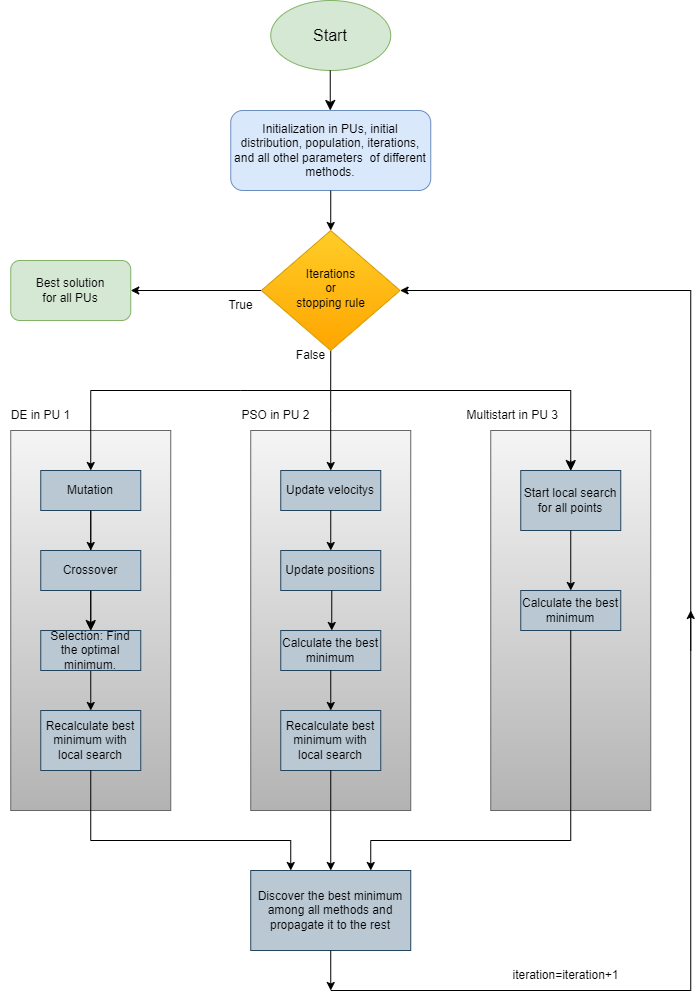
\includegraphics[scale=0.5]{pm_datagram}\caption{Flowchart of the overall process\label{fig:basicFlowchart}. The DE
acronym stands for the Differential Evolution method, the PU acronym
represents the Parallel Unit that executes the algorithm.}
\end{figure}


\section{Experiments\label{sec:Experiments}}

All experiments conducted were repeated 30 times to ensure the reliability
of the algorithm producing the results. In experimental research,
the number of repetitions required to ensure reliable results depends
on the nature of the experiment, the variability of the data, and
the precision requirements. There is no universal answer that applies
to all experiments, but general guidelines and best practices have
been established in the literature. In many scientific studies, at
least 30 repetitions are recommended to achieve satisfactory statistical
power. This is based on statistical theories such as the Law of Large
Numbers and theorems for estimating sample distributions. The initial
sample distribution is the same across all optimization methods, and
the other parameters have been kept constant, as shown in Table \ref{tab:settings}.
Specifically, in the parallel algorithm, the total number of initial
samples remains as constant as possible, regardless of the number
of threads used. The parallelization was achieved using the OpenMP
library \citep{openMP}, while the implementation of the method was
done in ANSI C++ within the optimization package OPTIMUS, available
at \url{https://github.com/itsoulos/OPTIMUS}. The parameters used
here are either suggested in the original publications of the methods
(eg Differential Evolution, Particle Swarm Optimization) or have been
chosen so that there is a compromise between the execution time of
the method and its efficiency.

\begin{table}[H]
\centering{}\caption{The following parameters were considered for conducting the experiments\label{tab:settings}}
\begin{tabular}{>{\centering}p{3cm}>{\centering}p{5.8cm}c}
\toprule 
Parameter & Value & Explanation\tabularnewline
\midrule
\midrule 
$N_{p}$ & 120 & Total particles for PSO \tabularnewline
\midrule 
$N_{d}$ & 120 & Total elements for DE \tabularnewline
\midrule 
$N_{m}$ & 120 & Total elements for Multistart \tabularnewline
\midrule 
$N_{k}$ & 200 & Maximum number of iterations\tabularnewline
\midrule 
$N_{s}$ & 15 & Similarity max count\tabularnewline
\midrule 
$F$ & 0.8  & Differential weight for DE\tabularnewline
\midrule 
$CR$ & 0.9  & Crossover Probability for DE\tabularnewline
\midrule 
$P_{m}$ & 0.005 & Local search rate for DE and PSO\tabularnewline
\midrule 
$C_{1},C_{2}$ & 0.5 & Parameters of PSO\tabularnewline
\bottomrule
\end{tabular}
\end{table}


\subsection{Test functions}

The test functions \citep{Floudas,Montaz Ali} presented below exhibit
varying levels of difficulty in solving them; hence, a periodic local
optimization mechanism has been incorporated. Periodic local optimization
plays a crucial role in increasing the success rate in locating the
minimum of functions. This addition appears to lead to a success rate
approaching 100\% for all functions, regardless of their characteristics
such as dimensionality, minima, scalability, and symmetry. A study
by Z.-M. Gao and colleagues \citep{Gao} specifically examines the
issue of symmetry and asymmetry in the test functions. The test functions
used in the conducted experiments are shown in Table \ref{tab:The-test-functions}.
Generally, the region of attraction $A\left(x^{*}\right)$ of a local
minimum $x^{*}$ is defined as:
\begin{equation}
A\left(x^{*}\right)=\left\{ x:\ x\in S,\ L(x)=x^{*}\right\} 
\end{equation}
where $L(x)$ is a local search procedure, such as BFGS. Global optimization
methods, usually find points which are in the region of attraction
$A\left(x^{*}\right)$ of a local minimum $x^{*}$ but not necessarily
the local minimum itself. For this reason, at the end of their execution,
a local minimization method is applied in order to ensure the exact
finding of a local minimum. Of course, this does not imply that the
minimum that will be located will be the total minimum of the function,
since a function can contain tens or even hundreds of local minima. 

\begin{table}[H]
\caption{The test functions used in the conducted experiments.\label{tab:The-test-functions}}

\centering{}%
\begin{tabular}{|c|c|c|}
\hline 
{\footnotesize{}NAME} & {\scriptsize{}FORMULA} & {\scriptsize{}DIMENSION}\tabularnewline
\hline 
\hline 
{\footnotesize{}Bent Cigar} & {\scriptsize{}$f(x)=x_{1}^{2}+10^{6}\sum_{i=2}^{n}x_{i}^{2}$} & {\scriptsize{}10}\tabularnewline
\hline 
{\footnotesize{}BF1} & {\scriptsize{}$f(x)=x_{1}^{2}+2x_{2}^{2}-\frac{3}{10}\cos\left(3\pi x_{1}\right)-\frac{4}{10}\cos\left(4\pi x_{2}\right)+\frac{7}{10}$} & {\scriptsize{}2}\tabularnewline
\hline 
{\footnotesize{}BF2} & {\scriptsize{}$f(x)=x_{1}^{2}+2x_{2}^{2}-\frac{3}{10}\cos\left(3\pi x_{1}\right)\cos\left(4\pi x_{2}\right)+\frac{3}{10}$} & {\scriptsize{}2}\tabularnewline
\hline 
{\footnotesize{}Branin} & {\scriptsize{}$f(x)=\left(x_{2}-\frac{5.1}{4\pi^{2}}x_{1}^{2}+\frac{5}{\pi}x_{1}-6\right)^{2}+10\left(1-\frac{1}{8\pi}\right)\cos(x_{1})+10$} & {\scriptsize{}2}\tabularnewline
\hline 
{\footnotesize{}CM} & {\scriptsize{}$f(x)=\sum_{i=1}^{n}x_{i}^{2}-\frac{1}{10}\sum_{i=1}^{n}\cos\left(5\pi x_{i}\right)$} & {\scriptsize{}4}\tabularnewline
\hline 
{\footnotesize{}Discus} & {\scriptsize{}$f(x)=10^{6}x_{1}^{2}+\sum_{i=2}^{n}x_{i}^{2}$} & {\scriptsize{}10}\tabularnewline
\hline 
{\footnotesize{}Easom} & {\scriptsize{}$f(x)=-\cos\left(x_{1}\right)\cos\left(x_{2}\right)\exp\left(\left(x_{2}-\pi\right)^{2}-\left(x_{1}-\pi\right)^{2}\right)$} & {\scriptsize{}2}\tabularnewline
\hline 
{\footnotesize{}Exp} & {\scriptsize{}$f(x)=-\exp\left(-0.5\sum_{i=1}^{n}x_{i}^{2}\right),\quad-1\le x_{i}\le1$} & {\scriptsize{}$n=4,16$}\tabularnewline
\hline 
{\footnotesize{}Griewank2} & {\scriptsize{}$f(x)=1+\frac{1}{200}\sum_{i=1}^{2}x_{i}^{2}-\prod_{i=1}^{2}\frac{\cos(x_{i})}{\sqrt{(i)}}$} & {\scriptsize{}2}\tabularnewline
\hline 
{\footnotesize{}Griewank10} & {\scriptsize{}f$(x)=1+\frac{1}{200}\sum_{i=1}^{10}x_{i}^{2}-\prod_{i=1}^{10}\frac{\cos(x_{i})}{\sqrt{(i)}}$} & {\scriptsize{}10}\tabularnewline
\hline 
{\footnotesize{}Gkls\citep{Gaviano}} & {\scriptsize{}$f(x)=\mbox{Gkls}(x,n,w)$} & {\scriptsize{}$n=2,3\ w=50,100$}\tabularnewline
\hline 
{\footnotesize{}Hansen} & {\scriptsize{}$f(x)=\sum_{i=1}^{5}i\cos\left[(i-1)x_{1}+i\right]\sum_{j=1}^{5}j\cos\left[(j+1)x_{2}+j\right]$} & {\scriptsize{}2}\tabularnewline
\hline 
{\footnotesize{}Hartman3} & {\scriptsize{}$f(x)=-\sum_{i=1}^{4}c_{i}\exp\left(-\sum_{j=1}^{3}a_{ij}\left(x_{j}-p_{ij}\right)^{2}\right)$} & {\scriptsize{}3}\tabularnewline
\hline 
{\footnotesize{}Hartman6} & {\scriptsize{}$f(x)=-\sum_{i=1}^{4}c_{i}\exp\left(-\sum_{j=1}^{6}a_{ij}\left(x_{j}-p_{ij}\right)^{2}\right)$} & {\scriptsize{}6}\tabularnewline
\hline 
{\footnotesize{}High Elliptic} & {\scriptsize{}$f(x)=\sum_{i=1}^{n}\left(10^{6}\right)^{\frac{i-1}{n-1}}x_{i}^{2}$} & {\scriptsize{}10}\tabularnewline
\hline 
{\footnotesize{}Potential\citep{Lennard}} & {\scriptsize{}$V_{LJ}(r)=4\epsilon\left[\left(\frac{\sigma}{r}\right)^{12}-\left(\frac{\sigma}{r}\right)^{6}\right]$} & {\scriptsize{}$n=9,15,21,30$}\tabularnewline
\hline 
{\footnotesize{}Rastrigin} & {\scriptsize{}$f(x)=x_{1}^{2}+x_{2}^{2}-\cos(18x_{1})-\cos(18x_{2})$} & {\scriptsize{}2}\tabularnewline
\hline 
{\footnotesize{}Shekel5} & {\scriptsize{}$f(x)=-\sum_{i=1}^{5}\frac{1}{(x-a_{i})(x-a_{i})^{T}+c_{i}}$} & {\scriptsize{}4}\tabularnewline
\hline 
{\footnotesize{}Shekel7} & {\scriptsize{}$f(x)=-\sum_{i=1}^{7}\frac{1}{(x-a_{i})(x-a_{i})^{T}+c_{i}}$} & {\scriptsize{}4}\tabularnewline
\hline 
{\footnotesize{}Shekel10} & {\scriptsize{}$f(x)=-\sum_{i=1}^{10}\frac{1}{(x-a_{i})(x-a_{i})^{T}+c_{i}}$} & {\scriptsize{}4}\tabularnewline
\hline 
{\footnotesize{}Sinusoidal\citep{Zabinsky}} & {\scriptsize{}$f(x)=-\left(2.5\prod_{i=1}^{n}\sin\left(x_{i}-z\right)+\prod_{i=1}^{n}\sin\left(5\left(x_{i}-z\right)\right)\right),\quad0\le x_{i}\le\pi$} & {\scriptsize{}$n=4,8$}\tabularnewline
\hline 
{\footnotesize{}Test2N} & {\scriptsize{}$f(x)=\frac{1}{2}\sum_{i=1}^{n}x_{i}^{4}-16x_{i}^{2}+5x_{i}$} & {\scriptsize{}$n=4,9$}\tabularnewline
\hline 
{\footnotesize{}Test30N} & {\scriptsize{}$\frac{1}{10}\sin^{2}\left(3\pi x_{1}\right)\sum_{i=2}^{n-1}\left(\left(x_{i}-1\right)^{2}\left(1+\sin^{2}\left(3\pi x_{i+1}\right)\right)\right)+\left(x_{n}-1\right)^{2}\left(1+\sin^{2}\left(2\pi x_{n}\right)\right)$} & {\scriptsize{}$n=3,4$}\tabularnewline
\hline 
\end{tabular}
\end{table}


\subsection{Experimental results}

All tables presented here demonstrate the average function calls obtained
for each test problem. The average function can be considered as a
measure of the speed of each method, since each function has a different
complexity and therefore, the average execution time would not be
a good indication of the computational time required. In the first
set of experiments we examined if the presence of the suggested stopping
rule, which is the combination of a series of stopping rules, affects
the optimization techniques without parallelization. During parallel
execution, the total sum of calls is computed across all computing
units nodes, ensuring efficient load distribution and resource utilization.
However, the algorithm terminates at the computing unit that identifies
the optimal solution, signaling the achievement of the desired convergence
criterion. In Table \ref{tab:DE}, we observe the performance of all
termination rules for the DE method. From these, both statistical
and quantitative comparisons arise, depicted in Figure \ref{fig:DE_stat}. 

\begin{table}[H]
\centering{}\caption{Average function calls for the Differential evolution method, using
different  termination rules\label{tab:DE}}
\begin{tabular}{|l|c|c|c|c|}
\hline 
\textbf{Problem} & \textbf{BEST} & \textbf{MEAN} & \textbf{DOUBLEBOX} & \textbf{ALL}\tabularnewline
\hline 
\hline 
\textbf{BF1} & 6761 & 10511 & 10369 & 6114\tabularnewline
\hline 
\textbf{BF2} & 7693 & 9222 & 11524 & 7560\tabularnewline
\hline 
\textbf{BRANIN} & 4639 & 10982 & 4907 & 4289\tabularnewline
\hline 
\textbf{CAMEL} & 6116 & 13290 & 9905 & 5940\tabularnewline
\hline 
\textbf{CIGAR10} & 7647 & 4348 & 21116 & 3111\tabularnewline
\hline 
\textbf{CM4} & 7913 & 4175 & 11851 & 4079\tabularnewline
\hline 
\textbf{DISCUS10} & 5191 & 2042 & 13614 & 2034\tabularnewline
\hline 
\textbf{EASOM} & 1917 & 15103 & 1721 & 1721\tabularnewline
\hline 
\textbf{ELP10} & 6046 & 24675 & 12519 & 6031\tabularnewline
\hline 
\textbf{EXP4} & 5216 & 18151 & 6385 & 5040\tabularnewline
\hline 
\textbf{EXP16} & 5588 & 27387 & 7552 & 5339\tabularnewline
\hline 
\textbf{GKLS250} & 5227 & 2641 & 8379 & 2641\tabularnewline
\hline 
\textbf{GKLS350} & 5624 & 3298 & 17437 & 3206\tabularnewline
\hline 
\textbf{GRIEWANK2} & 8027 & 10458 & 14756 & 6915\tabularnewline
\hline 
\textbf{GRIEWANK10} & 9664 & 37839 & 17312 & 9539\tabularnewline
\hline 
\textbf{POTENTIAL3} & 5278 & 24823 & 13871 & 5256\tabularnewline
\hline 
\textbf{PONTENTIAL5} & 8225 & 32439 & 20828 & 7742\tabularnewline
\hline 
\textbf{PONTENTIAL6} & 8467 & 34946 & 19169 & 8197\tabularnewline
\hline 
\textbf{PONTENTIAL10} & 10330 & 41300 & 26308 & 10643\tabularnewline
\hline 
\textbf{HANSEN} & 5219 & 23050 & 14245 & 4263\tabularnewline
\hline 
\textbf{HARTMAN3} & 4613 & 17966 & 7333 & 4566\tabularnewline
\hline 
\textbf{HARTMAN6} & 5734 & 17109 & 9354 & 5550\tabularnewline
\hline 
\textbf{RASTRIGIN} & 5912 & 17240 & 8987 & 5999\tabularnewline
\hline 
\textbf{ROSENBROCK8} & 8503 & 34429 & 20980 & 8051\tabularnewline
\hline 
\textbf{ROSENBROCK16} & 10052 & 41335 & 26156 & 8307\tabularnewline
\hline 
\textbf{SHEKEL5} & 6064 & 25800 & 19877 & 5933\tabularnewline
\hline 
\textbf{SHEKEL7} & 5597 & 26168 & 20274 & 5677\tabularnewline
\hline 
\textbf{SHEKEL10} & 6037 & 26439 & 22960 & 5100\tabularnewline
\hline 
\textbf{SINU4} & 5751 & 24620 & 12511 & 4776\tabularnewline
\hline 
\textbf{SINU8} & 6340 & 25477 & 18741 & 4980\tabularnewline
\hline 
\textbf{TEST2N4} & 5848 & 24947 & 11640 & 5727\tabularnewline
\hline 
\textbf{TEST2N9} & 7303 & 26571 & 16165 & 6288\tabularnewline
\hline 
\textbf{TEST30N3} & 3169 & 8395 & 8134 & 2869\tabularnewline
\hline 
\textbf{TEST30N4} & 2841 & 10381 & 7853 & 2714\tabularnewline
\hline 
\textbf{Total} & \textbf{214552} & \textbf{677557} & \textbf{474733} & \textbf{186197}\tabularnewline
\hline 
\end{tabular}
\end{table}

\begin{figure}[H]
\begin{centering}
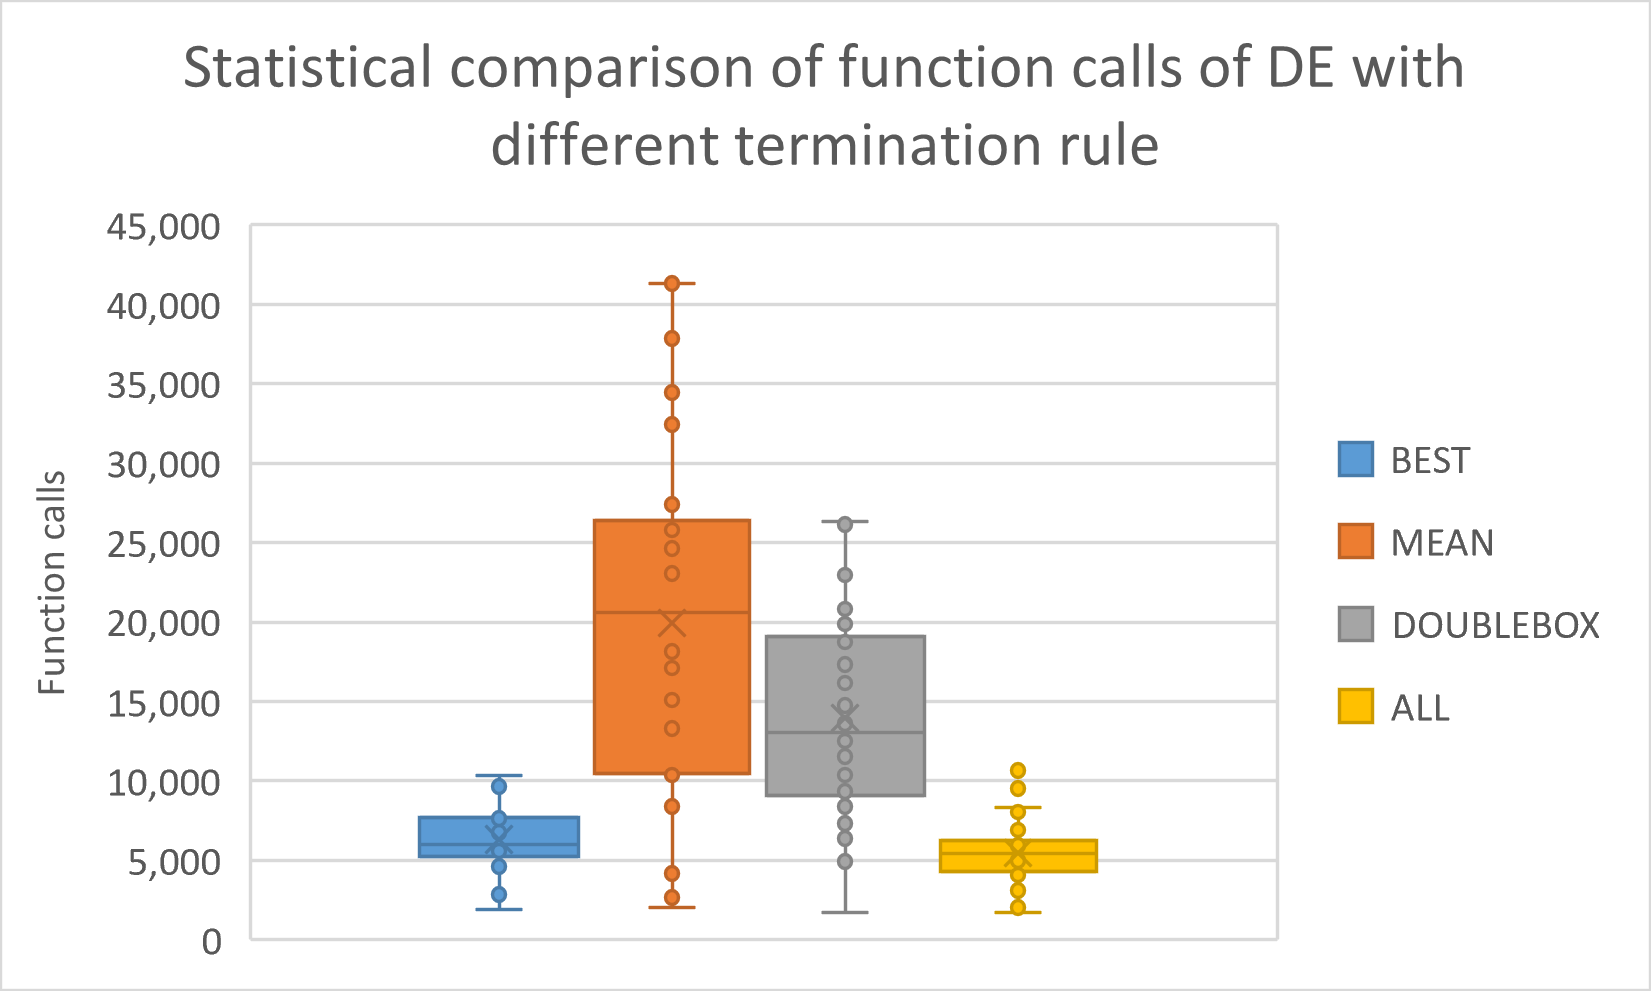
\includegraphics{table3}
\par\end{centering}
\centering{}\caption{Statistical comparison of function calls with different termination
rule of differential evolution\label{fig:DE_stat}}
\end{figure}
As it is evident, the combination of the stopping rules reduces the
required number of function calls that are required to obtain the
global minimum by the DE method. The proposed termination scheme outperforms
by a percentage that varies from 13\% to 73\% the other termination
rules used here. Subsequently, the same experiment was conducted for
the PSO method and the results are shown in Table \ref{tab:PSO} and
the statistical comparison is outlined graphically in Figure \ref{fig:PSO_stat}.

\begin{table}[H]
\centering{}\caption{Average function calls for the PSO method, with different termination
rules\label{tab:PSO}}
\begin{tabular}{|l|c|c|c|c|}
\hline 
\textbf{Problem} & \textbf{BEST} & \textbf{MEAN} & \textbf{DOUBLEBOX} & \textbf{ALL}\tabularnewline
\hline 
\hline 
\textbf{BF1} & 3418 & 3127 & 3122 & 3005\tabularnewline
\hline 
\textbf{BF2} & 3265 & 2995 & 2919 & 2889\tabularnewline
\hline 
\textbf{BRANIN} & 2601 & 2549 & 2431 & 2417\tabularnewline
\hline 
\textbf{CAMEL} & 2801 & 2675 & 2547 & 2547\tabularnewline
\hline 
\textbf{CIGAR10} & 3987 & 3674 & 3638 & 3638\tabularnewline
\hline 
\textbf{CM4} & 3863 & 3299 & 3144 & 3144\tabularnewline
\hline 
\textbf{DISCUS10} & 2611 & 2409 & 2405 & 2405\tabularnewline
\hline 
\textbf{EASOM} & 2420 & 2232 & 2232 & 2232\tabularnewline
\hline 
\textbf{ELP10} & 1705 & 1741 & 1586 & 1586\tabularnewline
\hline 
\textbf{EXP4} & 2751 & 2558 & 2558 & 2558\tabularnewline
\hline 
\textbf{EXP16} & 2898 & 2676 & 2676 & 2676\tabularnewline
\hline 
\textbf{GKLS250} & 2796 & 2553 & 2422 & 2422\tabularnewline
\hline 
\textbf{GKLS350} & 2947 & 2645 & 3833 & 2558\tabularnewline
\hline 
\textbf{GRIEWANK2} & 4405 & 2839 & 4282 & 2820\tabularnewline
\hline 
\textbf{GRIEWANK10} & 5327 & 4561 & 4797 & 4248\tabularnewline
\hline 
\textbf{POTENTIAL3} & 3289 & 3231 & 3222 & 3170\tabularnewline
\hline 
\textbf{PONTENTIAL5} & 4926 & 4881 & 7282 & 4730\tabularnewline
\hline 
\textbf{PONTENTIAL6} & 6699 & 5537 & 7534 & 5077\tabularnewline
\hline 
\textbf{PONTENTIAL10} & 10582 & 6737 & 29865 & 6539\tabularnewline
\hline 
\textbf{HANSEN} & 3788 & 2687 & 3062 & 2587\tabularnewline
\hline 
\textbf{HARTMAN3} & 2807 & 2743 & 2550 & 2550\tabularnewline
\hline 
\textbf{HARTMAN6} & 3081 & 2915 & 2809 & 2809\tabularnewline
\hline 
\textbf{RASTRIGIN} & 3558 & 2990 & 2829 & 2829\tabularnewline
\hline 
\textbf{ROSENBROCK8} & 4279 & 4263 & 4036 & 3969\tabularnewline
\hline 
\textbf{ROSENBROCK16} & 5761 & 5432 & 5170 & 5170\tabularnewline
\hline 
\textbf{SHEKEL5} & 3132 & 2823 & 12476 & 2816\tabularnewline
\hline 
\textbf{SHEKEL7} & 3064 & 2855 & 11520 & 2856\tabularnewline
\hline 
\textbf{SHEKEL10} & 3128 & 2942 & 14786 & 2866\tabularnewline
\hline 
\textbf{SINU4} & 3047 & 2740 & 2673 & 2657\tabularnewline
\hline 
\textbf{SINU8} & 3177 & 2824 & 4113 & 2828\tabularnewline
\hline 
\textbf{TEST2N4} & 3037 & 2839 & 2681 & 2681\tabularnewline
\hline 
\textbf{TEST2N9} & 4188 & 3106 & 3105 & 3067\tabularnewline
\hline 
\textbf{TEST30N3} & 2943 & 3130 & 2762 & 2762\tabularnewline
\hline 
\textbf{TEST30N4} & 3202 & 3185 & 2915 & 2915\tabularnewline
\hline 
\textbf{Total} & \textbf{125483} & \textbf{110393} & \textbf{169982} & \textbf{106023}\tabularnewline
\hline 
\end{tabular}
\end{table}

\begin{figure}[H]
\begin{centering}
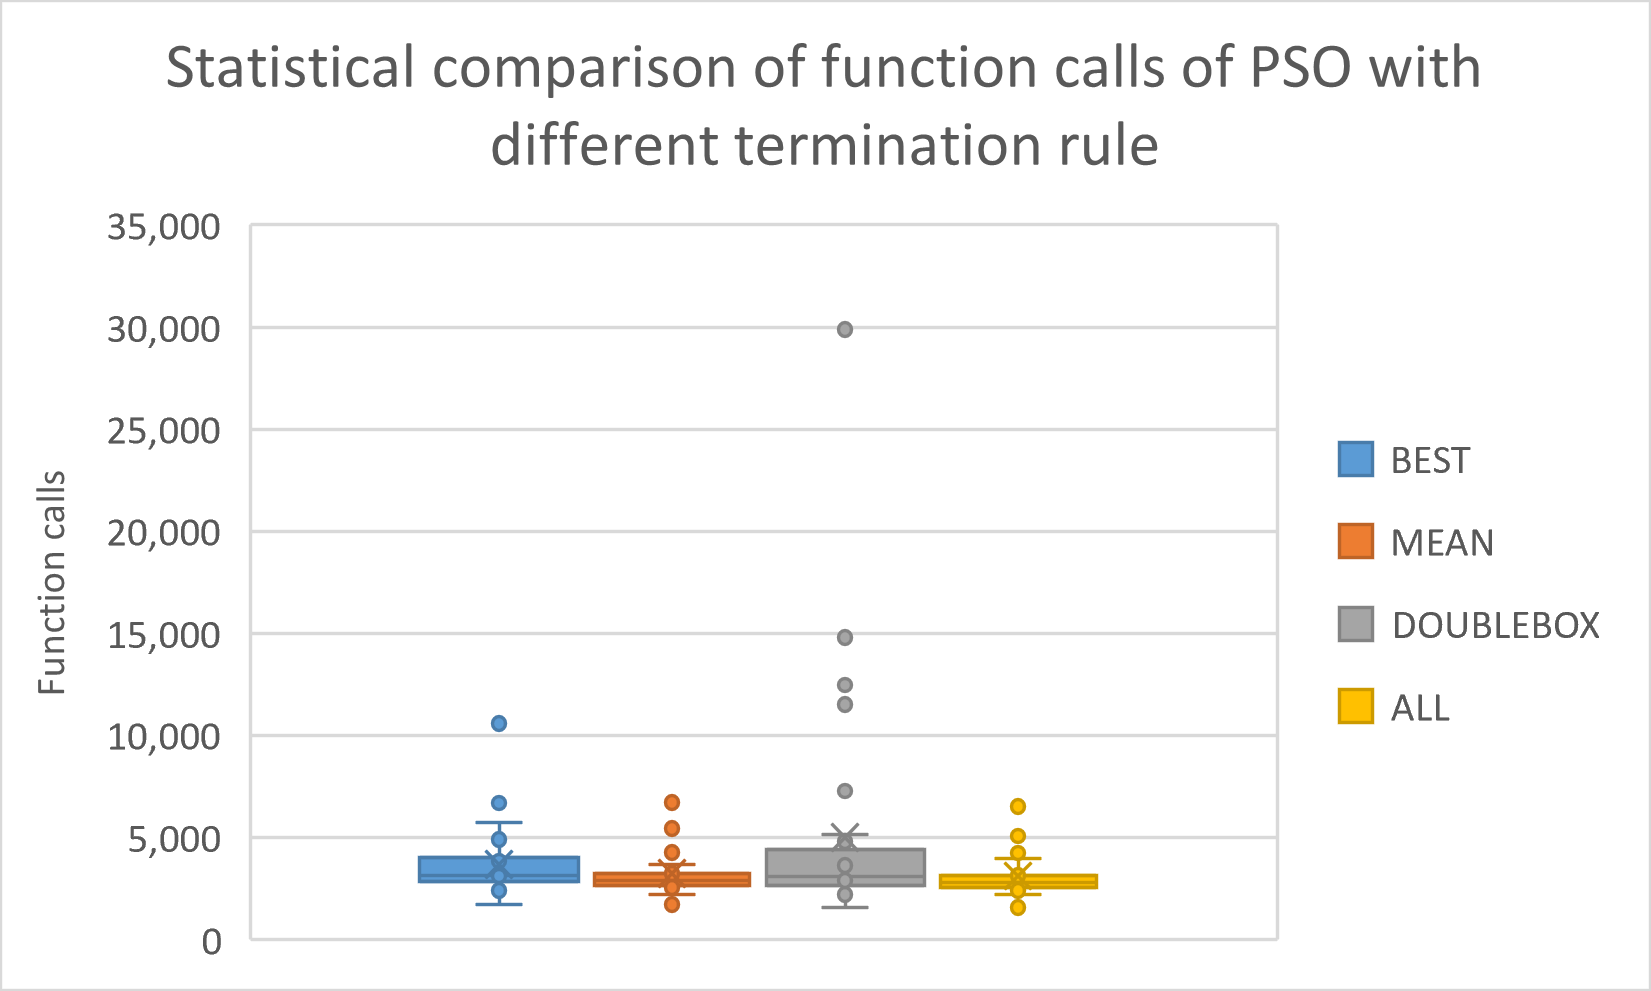
\includegraphics{table4}
\par\end{centering}
\caption{Statistical comparison of function calls with different termination
rule of PSO method\label{fig:PSO_stat}}
\end{figure}
Once more, the proposed termination scheme outperforms the other stopping
rules in almost every test function. Likewise, the same experiment
was carried out for the Multistart method and the results are depicted
in Table \ref{tab:Multistart} and the statistical comparison is shown
in Figure \ref{fig:Multistart_stat}.

\begin{table}[H]
\begin{centering}
\caption{Multistart: Function calls with different termination rules\label{tab:Multistart}}
\begin{tabular}{|l|c|c|c|c|}
\hline 
\textbf{Problem} & \textbf{BEST} & \textbf{MEAN} & \textbf{DOUBLEBOX} & \textbf{ALL}\tabularnewline
\hline 
\hline 
\textbf{BF1} & 53873 & 479374 & 50762 & 50762\tabularnewline
\hline 
\textbf{BF2} & 37670 & 239220 & 35711 & 35711\tabularnewline
\hline 
\textbf{BRANIN} & 11063 & 11046 & 10521 & 10521\tabularnewline
\hline 
\textbf{CAMEL} & 16083 & 153559 & 15255 & 15255\tabularnewline
\hline 
\textbf{CIGAR10} & 14937 & 14937 & 14697 & 14697\tabularnewline
\hline 
\textbf{CM4} & 62236 & 62192 & 58581 & 58581\tabularnewline
\hline 
\textbf{DISCUS10} & 6296 & 6296 & 6056 & 6056\tabularnewline
\hline 
\textbf{EASOM} & 5412 & 55130 & 51132 & 5412\tabularnewline
\hline 
\textbf{ELP10} & 14757 & 14981 & 14517 & 14517\tabularnewline
\hline 
\textbf{EXP4} & 10022 & 54174 & 9774 & 9774\tabularnewline
\hline 
\textbf{EXP16} & 10528 & 54680 & 10280 & 10280\tabularnewline
\hline 
\textbf{GKLS250} & 6202 & 47948 & 5908 & 5908\tabularnewline
\hline 
\textbf{GKLS350} & 7560 & 42145 & 7087 & 7087\tabularnewline
\hline 
\textbf{GRIEWANK2} & 19179 & 188429 & 17877 & 17877\tabularnewline
\hline 
\textbf{GRIEWANK10} & 65206 & 567153 & 61818 & 61818\tabularnewline
\hline 
\textbf{POTENTIAL3} & 17773 & 126632 & 17161 & 17161\tabularnewline
\hline 
\textbf{PONTENTIAL5} & 31347 & 226873 & 30249 & 30249\tabularnewline
\hline 
\textbf{PONTENTIAL6} & 35457 & 247144 & 33883 & 33883\tabularnewline
\hline 
\textbf{PONTENTIAL10} & 44957 & 283230 & 43618 & 43618\tabularnewline
\hline 
\textbf{HANSEN} & 18568 & 201543 & 17541 & 17541\tabularnewline
\hline 
\textbf{HARTMAN3} & 17395 & 162934 & 16562 & 16562\tabularnewline
\hline 
\textbf{HARTMAN6} & 22010 & 179073 & 21015 & 21015\tabularnewline
\hline 
\textbf{RASTRIGIN} & 24696 & 275610 & 23015 & 23015\tabularnewline
\hline 
\textbf{ROSENBROCK8} & 17850 & 17850 & 17610 & 17610\tabularnewline
\hline 
\textbf{ROSENBROCK16} & 25300 & 25300 & 25060 & 25060\tabularnewline
\hline 
\textbf{SHEKEL5} & 17725 & 151648 & 16972 & 16972\tabularnewline
\hline 
\textbf{SHEKEL7} & 17894 & 154373 & 17127 & 17127\tabularnewline
\hline 
\textbf{SHEKEL10} & 17931 & 159825 & 17135 & 17135\tabularnewline
\hline 
\textbf{SINU4} & 16429 & 155634 & 15647 & 15647\tabularnewline
\hline 
\textbf{SINU8} & 19519 & 170167 & 18674 & 18674\tabularnewline
\hline 
\textbf{TEST2N4} & 16486 & 154092 & 15806 & 15806\tabularnewline
\hline 
\textbf{TEST2N9} & 22035 & 160651 & 20716 & 20716\tabularnewline
\hline 
\textbf{TEST30N3} & 16934 & 161628 & 16145 & 16145\tabularnewline
\hline 
\textbf{TEST30N4} & 16686 & 159753 & 15907 & 15907\tabularnewline
\hline 
\textbf{Total} & \textbf{758016} & \textbf{5165224} & \textbf{769819} & \textbf{724099}\tabularnewline
\hline 
\end{tabular}
\par\end{centering}
\end{table}

\begin{figure}[H]
\begin{centering}
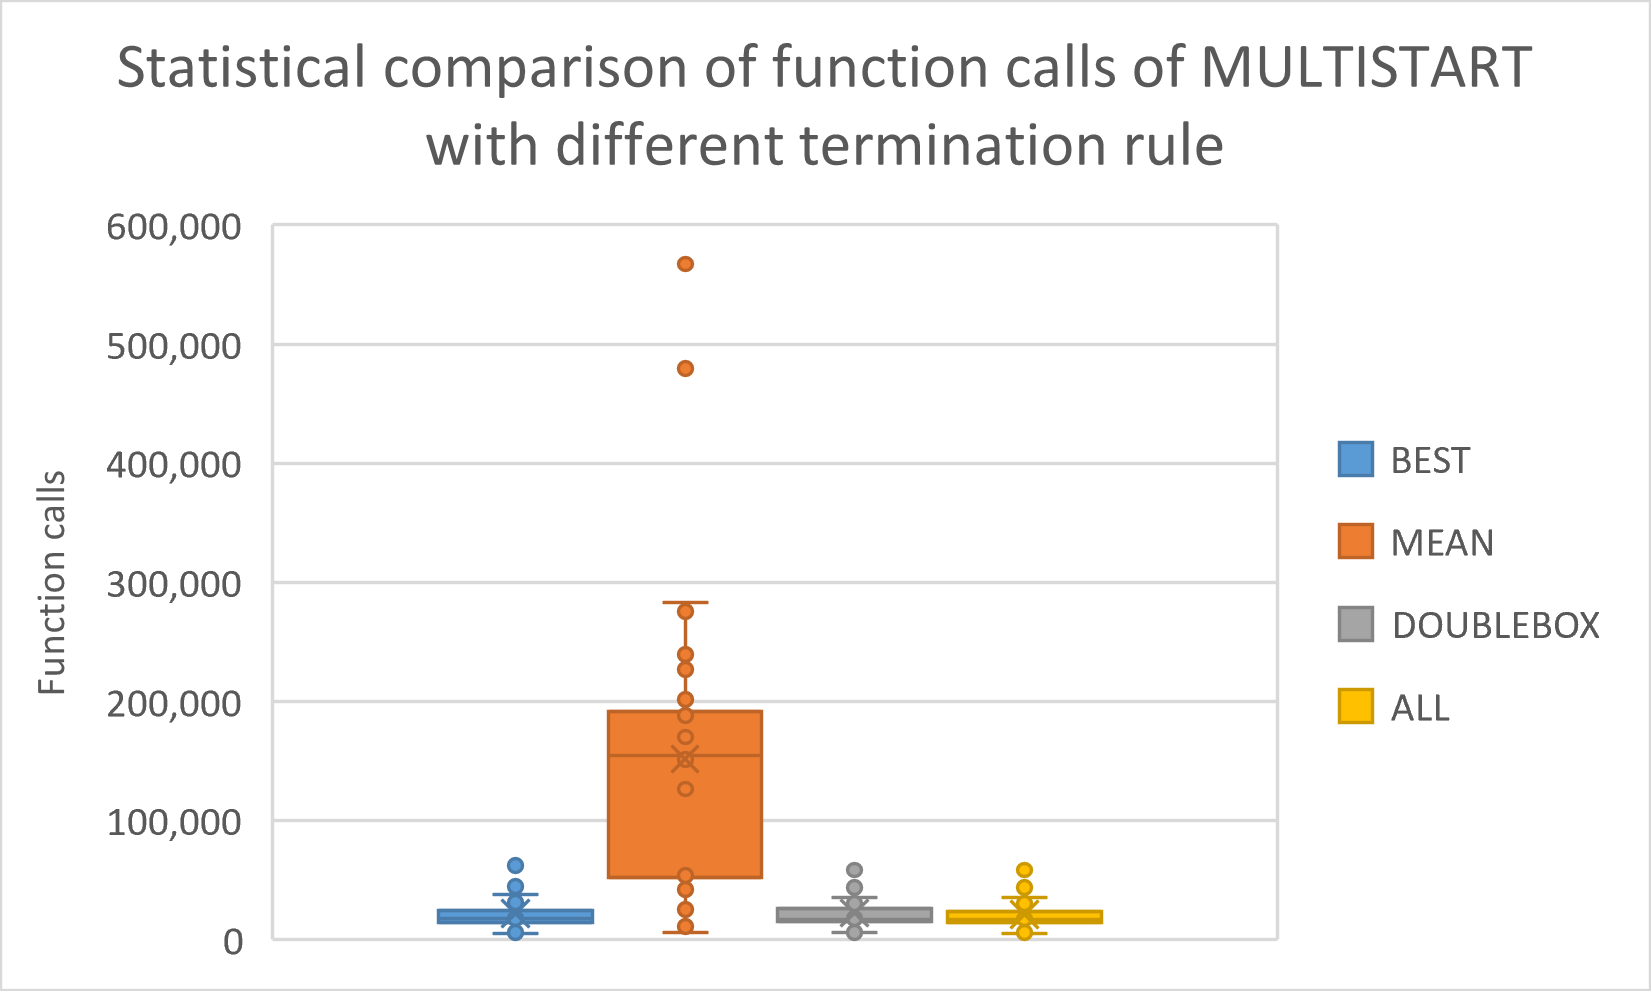
\includegraphics{table5}
\par\end{centering}
\begin{centering}
\caption{Statistical comparison of function calls with different termination
rule of multistart\label{fig:Multistart_stat}}
\par\end{centering}
\end{figure}
 Observing the tables with the corresponding statistical and quantitative
comparisons, it is evident that the calls to the objective function
for the proposed termination rule  are fewer than any other rule in
any method. Also, the proposed termination rule was also applied to
a recent global optimization method named Grey Wolf Optimizer \citep{gwo}
and the results are shown in Table \ref{tab:experGWO} and the corresponding
statistical comparison in Figure \ref{fig:experGWO}.

\begin{table}[H]
\caption{Experiments using the variety of termination rules and the GWO optimization
method.\label{tab:experGWO}}

\begin{centering}
\begin{tabular}{|l|c|c|c|c|}
\hline 
\textbf{Problem} & \textbf{BEST} & \textbf{MEAN} & \textbf{DOUBLEBOX} & \textbf{ALL}\tabularnewline
\hline 
\hline 
\textbf{BF1} & 3080 & 4675 & 6719 & 3080\tabularnewline
\hline 
\textbf{BF2} & 3083 & 4747 & 6923 & 3083\tabularnewline
\hline 
\textbf{BRANIN} & 3217 & 3217 & 5105 & 2661\tabularnewline
\hline 
\textbf{CAMEL} & 2750 & 3411 & 3780 & 2724\tabularnewline
\hline 
\textbf{CIGAR10} & 14718 & 23003 & 24134 & 14718\tabularnewline
\hline 
\textbf{CM4} & 3187 & 5638 & 8802 & 3187\tabularnewline
\hline 
\textbf{DISCUS10} & 12946 & 22194 & 24134 & 12946\tabularnewline
\hline 
\textbf{EASOM} & 2701 & 2965 & 10201 & 2135\tabularnewline
\hline 
\textbf{ELP10} & 6440 & 22449 & 24123 & 6440\tabularnewline
\hline 
\textbf{EXP4} & 2796 & 5198 & 7830 & 2796\tabularnewline
\hline 
\textbf{EXP16} & 4991 & 10842 & 22025 & 4991\tabularnewline
\hline 
\textbf{GKLS250} & 3072 & 3072 & 4840 & 2940\tabularnewline
\hline 
\textbf{GKLS350} & 4041 & 4041 & 8620 & 4041\tabularnewline
\hline 
\textbf{GRIEWANK2} & 3155 & 4818 & 7258 & 3155\tabularnewline
\hline 
\textbf{GRIEWANK10} & 8568 & 10196 & 22841 & 8568\tabularnewline
\hline 
\textbf{POTENTIAL3} & 3766 & 3766 & 13063 & 3701\tabularnewline
\hline 
\textbf{PONTENTIAL5} & 4082 & 4082 & 19826 & 3645\tabularnewline
\hline 
\textbf{PONTENTIAL6} & 3754 & 3754 & 19477 & 3380\tabularnewline
\hline 
\textbf{PONTENTIAL10} & 3502 & 3502 & 13129 & 2538\tabularnewline
\hline 
\textbf{HANSEN} & 3407 & 3407 & 8345 & 2795\tabularnewline
\hline 
\textbf{HARTMAN3} & 3251 & 3251 & 7587 & 2911\tabularnewline
\hline 
\textbf{HARTMAN6} & 3639 & 3639 & 13342 & 3408\tabularnewline
\hline 
\textbf{RASTRIGIN} & 2878 & 4499 & 6463 & 2806\tabularnewline
\hline 
\textbf{ROSENBROCK8} & 5859 & 22384 & 24123 & 5859\tabularnewline
\hline 
\textbf{ROSENBROCK16} & 8528 & 23513 & 24132 & 8528\tabularnewline
\hline 
\textbf{SHEKEL5} & 3381 & 3381 & 16781 & 2778\tabularnewline
\hline 
\textbf{SHEKEL7} & 3600 & 3600 & 17989 & 3324\tabularnewline
\hline 
\textbf{SHEKEL10} & 3258 & 3258 & 19227 & 2866\tabularnewline
\hline 
\textbf{SINU4} & 2923 & 2923 & 9767 & 2231\tabularnewline
\hline 
\textbf{SINU8} & 2934 & 2934 & 10714 & 2502\tabularnewline
\hline 
\textbf{TEST2N4} & 3623 & 3623 & 9619 & 3603\tabularnewline
\hline 
\textbf{TEST2N9} & 4327 & 4327 & 21381 & 4207\tabularnewline
\hline 
\textbf{TEST30N3} & 3225 & 3237 & 3513 & 2769\tabularnewline
\hline 
\textbf{TEST30N4} & 3324 & 3324 & 6124 & 3144\tabularnewline
\hline 
\textbf{Total} & \textbf{152006} & \textbf{236870} & \textbf{451937} & \textbf{144460}\tabularnewline
\hline 
\end{tabular}
\par\end{centering}
\end{table}
\begin{figure}[H]
\begin{centering}
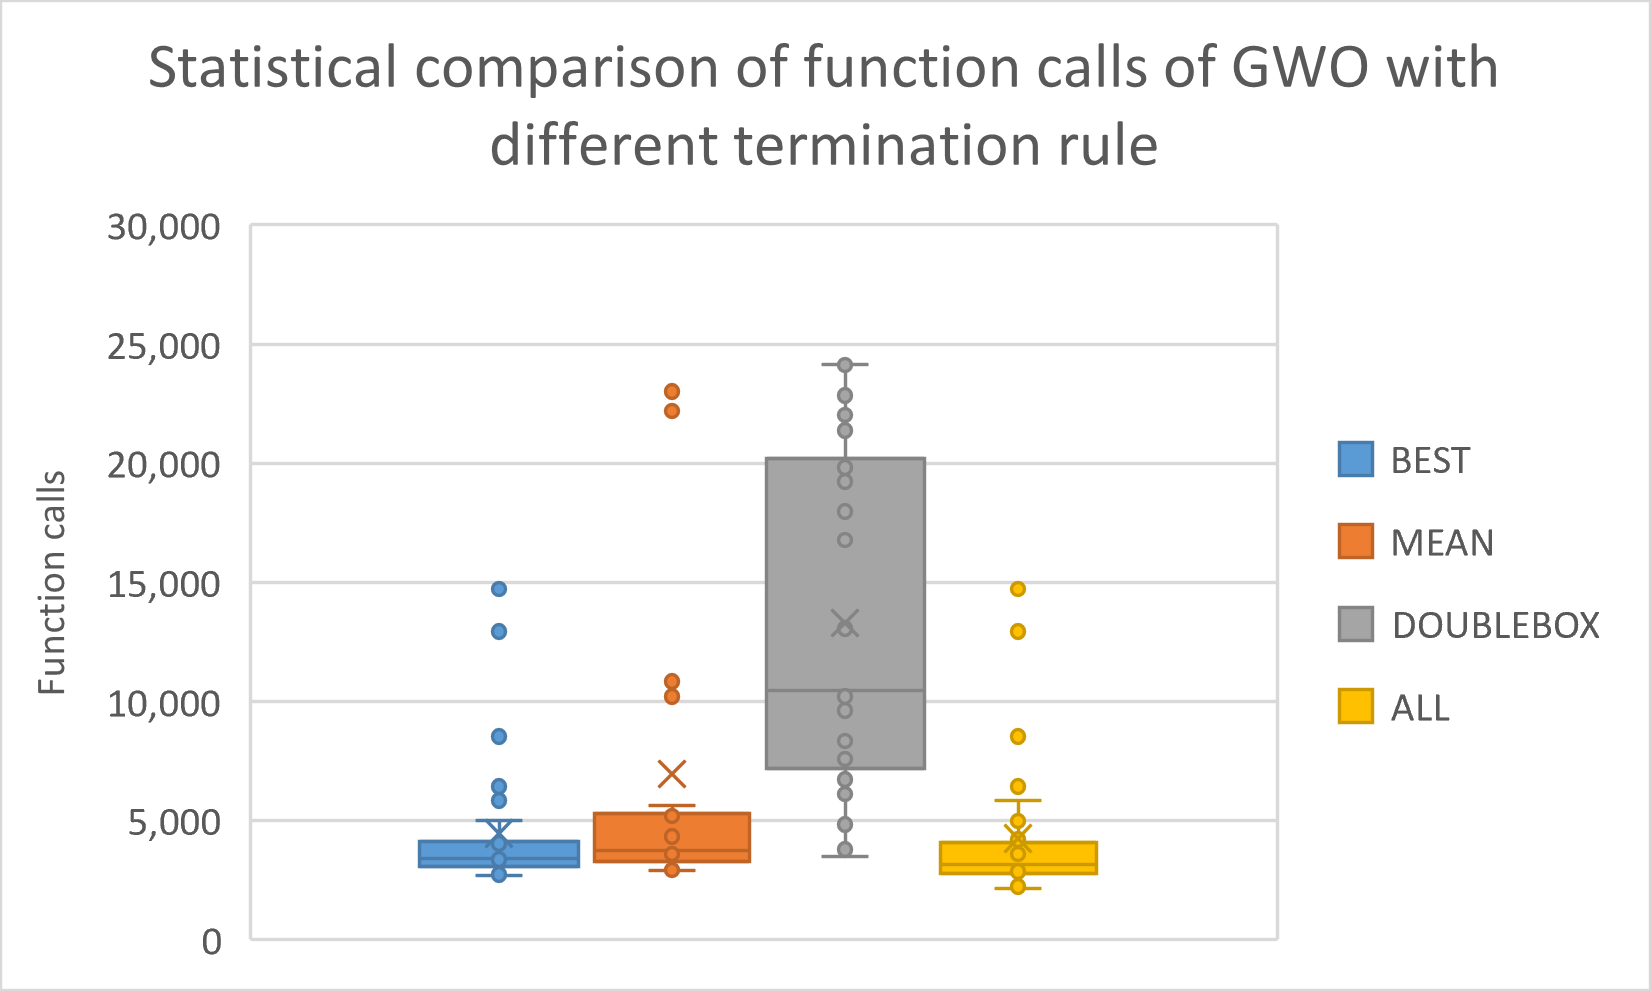
\includegraphics{table6}
\par\end{centering}
\caption{Statistical comparison for the GWO optimizer using different termination
rules.\label{fig:experGWO}}

\end{figure}
Once again the combinatorial termination technique achieves the lowest
number of function calls of all available techniques. Each optimization
method and termination criterion function differently and yield varying
results. This variation is further influenced by the differing nature
of the cost functions involved. When integrated into the overall algorithm,
each method, in combination with the termination criterion that best
suits it, can converge to optimal solutions more quickly, thereby
enhancing the algorithm's overall performance. 

The proposed termination rule was also applied to the current parallel
optimization technique for the test function described previously.
The experimental results for the so - called \emph{DoubleBox} stopping
rule and the given parallel method are show in Table \ref{tab:parallelDoublebox}.
The columns in the table stand for the following:
\begin{enumerate}
\item Column Problem denotes the test function used.
\item Column 1x500 denotes the application of the proposed technique with
one processing unit and 500 particles.
\item Column 2x250 stands for the usage of two processing units. In each
unit, the number of particles was set to 250.
\item Column 5x100 denotes the incorporation of 5 processing units into
the proposed method. In each processing unit the number of particles
was set to 100.
\item Column 10x50 stands for the usage of 10 processing units. In each
processing unit, the number of particles was set to 50.
\end{enumerate}
\begin{table}[H]
\centering{}\caption{Experiments using the proposed optimization technique and the Doublebox
stopping rule. The experiment was performed on the test functions
described previously. Numbers in cells denote average function calls.\label{tab:parallelDoublebox}}
\begin{tabular}{|c|c|c|c|c|}
\hline 
\textbf{Problem} & \textbf{1x500} & \textbf{2x250} & \textbf{5x100} & \textbf{10x50}\tabularnewline
\hline 
\hline 
\textbf{BF1} & 36018 & 28282 & 18419 & 10859\tabularnewline
\hline 
\textbf{BF2} & 42191 & 37555 & 16568 & 10710\tabularnewline
\hline 
\textbf{BRANIN} & 45165 & 45726 & 45757 & 34381\tabularnewline
\hline 
\textbf{CAMEL} & 54786 & 54782 & 54253 & 53839\tabularnewline
\hline 
\textbf{CIGAR10} & 18387 & 18300 & 18307 & 11950\tabularnewline
\hline 
\textbf{CM4} & 60796 & 60501 & 60287 & 60200\tabularnewline
\hline 
\textbf{DISCUS10} & 25115 & 24586 & 14565 & 8957\tabularnewline
\hline 
\textbf{EASOM} & 40376 & 40211 & 40100 & 40099\tabularnewline
\hline 
\textbf{ELP10} & 20193 & 14745 & 11211 & 7691\tabularnewline
\hline 
\textbf{EXP4} & 54779 & 54676 & 54416 & 54412\tabularnewline
\hline 
\textbf{EXP16} & 52768 & 52205 & 52563 & 52560\tabularnewline
\hline 
\textbf{GKLS250} & 51980 & 51240 & 51233 & 51231\tabularnewline
\hline 
\textbf{GKLS350} & 48577 & 48761 & 48702 & 4100\tabularnewline
\hline 
\textbf{GRIEWANK2} & 56767 & 56690 & 51170 & 26076\tabularnewline
\hline 
\textbf{GRIEWANK10} & 20941 & 20721 & 14870 & 11765\tabularnewline
\hline 
\textbf{POTENTIAL3} & 49418 & 49800 & 49109 & 49002\tabularnewline
\hline 
\textbf{PONTENTIAL5} & 59827 & 59656 & 59367 & 59322\tabularnewline
\hline 
\textbf{PONTENTIAL6} & 62720 & 62398 & 62294 & 62280\tabularnewline
\hline 
\textbf{PONTENTIAL10} & 72899 & 72745 & 72943 & 72578\tabularnewline
\hline 
\textbf{HANSEN} & 45064 & 45689 & 45510 & 45424\tabularnewline
\hline 
\textbf{HARTMAN3} & 47307 & 47112 & 47111 & 47100\tabularnewline
\hline 
\textbf{HARTMAN6} & 49370 & 49302 & 49312 & 49222\tabularnewline
\hline 
\textbf{RASTRIGIN} & 57617 & 56577 & 56513 & 56400\tabularnewline
\hline 
\textbf{ROSENBROCK8} & 22997 & 22903 & 14139 & 14001\tabularnewline
\hline 
\textbf{POSENBROCK16} & 42117 & 34856 & 21392 & 13722\tabularnewline
\hline 
\textbf{SHEKEL5} & 50631 & 50198 & 50233 & 44662\tabularnewline
\hline 
\textbf{SHEKEL7} & 51212 & 51200 & 51200 & 45610\tabularnewline
\hline 
\textbf{SHEKEL10} & 51741 & 51607 & 51587 & 47761\tabularnewline
\hline 
\textbf{SINU4} & 48140 & 48100 & 48111 & 48099\tabularnewline
\hline 
\textbf{SINU8} & 48761 & 48434 & 48423 & 48204\tabularnewline
\hline 
\textbf{TEST2N4} & 48904 & 48307 & 48354 & 48354\tabularnewline
\hline 
\textbf{TEST2N9} & 48838 & 48555 & 48600 & 48335\tabularnewline
\hline 
\textbf{TEST30N3} & 51640 & 51307 & 51194 & 51143\tabularnewline
\hline 
\textbf{TEST30N4} & 48992 & 48549 & 48540 & 48487\tabularnewline
\hline 
\textbf{Total} & \textbf{1587034} & \textbf{1556276} & \textbf{1476353} & \textbf{1338536}\tabularnewline
\hline 
\end{tabular}
\end{table}
In this experiment, the total number of particles was set to 500,
in order to have credibility in the values recorded. The results indicate
that the increase in processing units may reduce the required number
of function calls. The same series of experiments was also conducted
using the so - called \emph{mean fitness} termination rule, that has
been described in equation \ref{eq:mean}. The obtained results are
presented in Table \ref{tab:parallelMean}. 

\begin{table}[H]
\begin{centering}
\caption{Experiments using the proposed optimization technique and the mean
- fitness stopping rule. Numbers in cells denote average function
calls.\label{tab:parallelMean}}
\par\end{centering}
\centering{}%
\begin{tabular}{|c|c|c|c|c|}
\hline 
\textbf{Problems} & \textbf{1x500} & \textbf{2x250} & \textbf{5x100} & \textbf{10x50}\tabularnewline
\hline 
\hline 
\textbf{BF1} & 49714 & 41284 & 41089 & 19596\tabularnewline
\hline 
\textbf{BF2} & 58272 & 46270 & 41324 & 15878\tabularnewline
\hline 
\textbf{BRANIN} & 45165 & 45665 & 44894 & 7268\tabularnewline
\hline 
\textbf{CAMEL} & 54786 & 54989 & 54651 & 10295\tabularnewline
\hline 
\textbf{CIGAR10} & 63026 & 62206 & 60277 & 27217\tabularnewline
\hline 
\textbf{CM4} & 60796 & 60333 & 40072 & 12977\tabularnewline
\hline 
\textbf{DISCUS10} & 50988 & 50690 & 36151 & 14040\tabularnewline
\hline 
\textbf{EASOM} & 40376 & 34178 & 21355 & 7377\tabularnewline
\hline 
\textbf{ELP10} & 50397 & 16787 & 9334 & 7809\tabularnewline
\hline 
\textbf{EXP4} & 54749 & 54445 & 29812 & 11024\tabularnewline
\hline 
\textbf{EXP16} & 52768 & 51233 & 24782 & 10722\tabularnewline
\hline 
\textbf{GKLS250} & 51980 & 50333 & 37696 & 9641\tabularnewline
\hline 
\textbf{GKLS350} & 48577 & 48442 & 28420 & 9337\tabularnewline
\hline 
\textbf{GRIEWANK2} & 56767 & 40471 & 30632 & 12356\tabularnewline
\hline 
\textbf{GRIEWANK10} & 68439 & 58410 & 53818 & 30317\tabularnewline
\hline 
\textbf{POTENTIAL3} & 49418 & 49328 & 33657 & 10140\tabularnewline
\hline 
\textbf{PONTENTIAL5} & 59827 & 58259 & 34436 & 11515\tabularnewline
\hline 
\textbf{PONTENTIAL6} & 62720 & 62715 & 34158 & 14417\tabularnewline
\hline 
\textbf{PONTENTIAL10} & 72899 & 72800 & 64964 & 16780\tabularnewline
\hline 
\textbf{HANSEN} & 45064 & 45582 & 32013 & 9318\tabularnewline
\hline 
\textbf{HARTMAN3} & 47307 & 47983 & 31033 & 8899\tabularnewline
\hline 
\textbf{HARTMAN6} & 49370 & 47983 & 27884 & 9602\tabularnewline
\hline 
\textbf{RASTRIGIN} & 54637 & 53551 & 33095 & 10169\tabularnewline
\hline 
\textbf{ROSENBROCK8} & 67885 & 57314 & 46961 & 25383\tabularnewline
\hline 
\textbf{POSENBROCK16} & 77207 & 66172 & 59098 & 41461\tabularnewline
\hline 
\textbf{SHEKEL5} & 50631 & 49800 & 32025 & 10389\tabularnewline
\hline 
\textbf{SHEKEL7} & 51212 & 50630 & 29136 & 11193\tabularnewline
\hline 
\textbf{SHEKEL10} & 51741 & 50321 & 33462 & 11200\tabularnewline
\hline 
\textbf{SINU4} & 48140 & 52788 & 32412 & 9721\tabularnewline
\hline 
\textbf{SINU8} & 48761 & 55864 & 32685 & 10410\tabularnewline
\hline 
\textbf{TEST2N4} & 48904 & 48800 & 28959 & 8643\tabularnewline
\hline 
\textbf{TEST2N9} & 48838 & 47001 & 36281 & 8085\tabularnewline
\hline 
\textbf{TEST30N3} & 51514 & 50100 & 39828 & 11699\tabularnewline
\hline 
\textbf{TEST30N4} & 48992 & 46875 & 42564 & 11954\tabularnewline
\hline 
\textbf{Total} & \textbf{1841867} & \textbf{1729602} & \textbf{1258958} & \textbf{456832}\tabularnewline
\hline 
\end{tabular}
\end{table}

\begin{table}
\caption{Experiments using the proposed optimization technique and the best
- fitness stopping rule. Numbers in cells denote average function
calls.\label{tab:parallelBest}}

\centering{}%
\begin{tabular}{|c|c|c|c|c|}
\hline 
Problems & 1x500 & 2x250 & 5x100 & 10x50\tabularnewline
\hline 
\hline 
BF1 & 9270 & 6253 & 6497 & 6089\tabularnewline
\hline 
BF2 & 9838 & 6249 & 6078 & 5853\tabularnewline
\hline 
BRANIN & 5787 & 5022 & 4991 & 4989\tabularnewline
\hline 
CAMEL & 12204 & 5882 & 5765 & 5399\tabularnewline
\hline 
CIGAR10 & 7631 & 6482 & 6350 & 6420\tabularnewline
\hline 
CM4 & 16222 & 5037 & 7422 & 6366\tabularnewline
\hline 
DISCUS10 & 5997 & 7364 & 4906 & 5037\tabularnewline
\hline 
EASOM & 4701 & 4752 & 4653 & 4668\tabularnewline
\hline 
ELP10 & 6230 & 5223 & 5407 & 5314\tabularnewline
\hline 
EXP4 & 10277 & 5675 & 5638 & 5526\tabularnewline
\hline 
EXP16 & 9577 & 5575 & 5471 & 5470\tabularnewline
\hline 
GKLS250 & 13328 & 5864 & 5323 & 4993\tabularnewline
\hline 
GKLS350 & 10131 & 4998 & 5442 & 4919\tabularnewline
\hline 
GRIEWANK2 & 8504 & 7345 & 6108 & 5876\tabularnewline
\hline 
GRIEWANK10 & 8535 & 7704 & 7771 & 7126\tabularnewline
\hline 
POTENTIAL3 & 11338 & 5726 & 5471 & 5699\tabularnewline
\hline 
PONTENTIAL5 & 12414 & 7192 & 6977 & 7070\tabularnewline
\hline 
PONTENTIAL6 & 14760 & 8480 & 7210 & 7511\tabularnewline
\hline 
PONTENTIAL10 & 17729 & 12218 & 10217 & 9439\tabularnewline
\hline 
HANSEN & 8379 & 5945 & 5023 & 4972\tabularnewline
\hline 
HARTMAN3 & 10674 & 5613 & 5703 & 5163\tabularnewline
\hline 
HARTMAN6 & 10841 & 5541 & 5485 & 5536\tabularnewline
\hline 
RASTRIGIN & 13657 & 6636 & 6129 & 5399\tabularnewline
\hline 
ROSENBROCK8 & 9456 & 6979 & 7165 & 7049\tabularnewline
\hline 
POSENBROCK16 & 9853 & 8620 & 8110 & 8379\tabularnewline
\hline 
SHEKEL5 & 10959 & 5437 & 5684 & 5616\tabularnewline
\hline 
SHEKEL7 & 10651 & 5715 & 5739 & 5486\tabularnewline
\hline 
SHEKEL10 & 1533 & 6064 & 5772 & 5516\tabularnewline
\hline 
SINU4 & 10291 & 6249 & 5426 & 5188\tabularnewline
\hline 
SINU8 & 9993 & 6847 & 6080 & 5582\tabularnewline
\hline 
TEST2N4 & 10242 & 6131 & 5837 & 5480\tabularnewline
\hline 
TEST2N9 & 12998 & 7402 & 6455 & 5702\tabularnewline
\hline 
TEST30N3 & 6228 & 5712 & 5723 & 5321\tabularnewline
\hline 
TEST30N4 & 5540 & 5437 & 5490 & 5484\tabularnewline
\hline 
Total & 335768 & 217369 & 207518 & 199637\tabularnewline
\hline 
\end{tabular}
\end{table}

And in this series of experiments, the columns of the table retain
the same meaning as in Table \ref{tab:parallelDoublebox}. Furthermore,
once again, it is observed that the increase in the number of computing
units significantly reduces the required number of function calls
to find the global minimum. Additionally, there is a significant reduction
in the number of function calls required to be compared to the previous
termination rule. Finally, the proposed termination rule is utilized
in the parallel optimization technique and the experimental results
are outlined in Table \ref{tab:parallelProposed}.

\begin{table}[H]
\begin{centering}
\caption{Experiments using the proposed optimization technique and proposed
stopping rule. Numbers in cells denote average function calls.\label{tab:parallelProposed}}
\par\end{centering}
\centering{}%
\begin{tabular}{|c|c|c|c|c|}
\hline 
\textbf{Problems} & \textbf{1x500} & \textbf{2x250} & \textbf{5x100} & \textbf{10x50}\tabularnewline
\hline 
\hline 
\textbf{BF1} & 10839 & 6543 & 6375 & 5933\tabularnewline
\hline 
\textbf{BF2} & 9838 & 6317 & 5978 & 5716\tabularnewline
\hline 
\textbf{BRANIN} & 5787 & 5003 & 5076 & 4936\tabularnewline
\hline 
\textbf{CAMEL} & 12204 & 5889 & 5703 & 5434\tabularnewline
\hline 
\textbf{CIGAR10} & 7631 & 6575 & 6582 & 6500\tabularnewline
\hline 
\textbf{CM4} & 16222 & 8935 & 6837 & 6392\tabularnewline
\hline 
\textbf{DISCUS10} & 5997 & 5039 & 5001 & 5252\tabularnewline
\hline 
\textbf{EASOM} & 4701 & 4791 & 4772 & 4751\tabularnewline
\hline 
\textbf{ELP10} & 6230 & 5363 & 5471 & 5205\tabularnewline
\hline 
\textbf{EXP4} & 10277 & 5542 & 5620 & 5533\tabularnewline
\hline 
\textbf{EXP16} & 9577 & 5518 & 5544 & 5532\tabularnewline
\hline 
\textbf{GKLS250} & 13328 & 5993 & 5205 & 5011\tabularnewline
\hline 
\textbf{GKLS350} & 10131 & 7373 & 5094 & 4869\tabularnewline
\hline 
\textbf{GRIEWANK2} & 8504 & 8284 & 6371 & 5761\tabularnewline
\hline 
\textbf{GRIEWANK10} & 8535 & 7585 & 7229 & 6922\tabularnewline
\hline 
\textbf{POTENTIAL3} & 11338 & 5666 & 5830 & 5695\tabularnewline
\hline 
\textbf{PONTENTIAL5} & 12414 & 7310 & 7126 & 6996\tabularnewline
\hline 
\textbf{PONTENTIAL6} & 14760 & 8450 & 7477 & 7561\tabularnewline
\hline 
\textbf{PONTENTIAL10} & 17729 & 11928 & 10431 & 9338\tabularnewline
\hline 
\textbf{HANSEN} & 8379 & 6862 & 4883 & 4970\tabularnewline
\hline 
\textbf{HARTMAN3} & 10674 & 5395 & 5219 & 5078\tabularnewline
\hline 
\textbf{HARTMAN6} & 10841 & 5486 & 5649 & 5348\tabularnewline
\hline 
\textbf{RASTRIGIN} & 13657 & 8283 & 5850 & 5292\tabularnewline
\hline 
\textbf{ROSENBROCK8} & 9456 & 6751 & 7232 & 6979\tabularnewline
\hline 
\textbf{POSENBROCK16} & 9853 & 7993 & 8377 & 8086\tabularnewline
\hline 
\textbf{SHEKEL5} & 10959 & 5749 & 5810 & 5884\tabularnewline
\hline 
\textbf{SHEKEL7} & 10651 & 5828 & 5843 & 5698\tabularnewline
\hline 
\textbf{SHEKEL10} & 1533 & 5863 & 6112 & 5588\tabularnewline
\hline 
\textbf{SINU4} & 10291 & 6427 & 5371 & 5251\tabularnewline
\hline 
\textbf{SINU8} & 9993 & 7139 & 6274 & 5583\tabularnewline
\hline 
\textbf{TEST2N4} & 10242 & 7516 & 5573 & 5129\tabularnewline
\hline 
\textbf{TEST2N9} & 12998 & 10137 & 6112 & 5566\tabularnewline
\hline 
\textbf{TEST30N3} & 6228 & 5512 & 5402 & 5485\tabularnewline
\hline 
\textbf{TEST30N4} & 5540 & 5749 & 5750 & 5350\tabularnewline
\hline 
\textbf{Total} & \textbf{337337} & \textbf{228794} & \textbf{207179} & \textbf{198624}\tabularnewline
\hline 
\end{tabular}
\end{table}
And in this case, it is observed that the increase of parallel processing
units significantly reduces the required number of function calls,
as in the two previous termination rules. However, the proposed termination
rule dramatically reduces the number of required function calls and
consequently the computation time compared to previous termination
rules. This reduction in fact intensifies as the number of computing
nodes increases. Also, for the same set of experiments, a statistical
test (Wilcoxon test) was conducted and the it is graphically presented
in Figure \ref{fig:Wilcoxon-rank-sum-test}.

\begin{figure}[H]
\begin{centering}
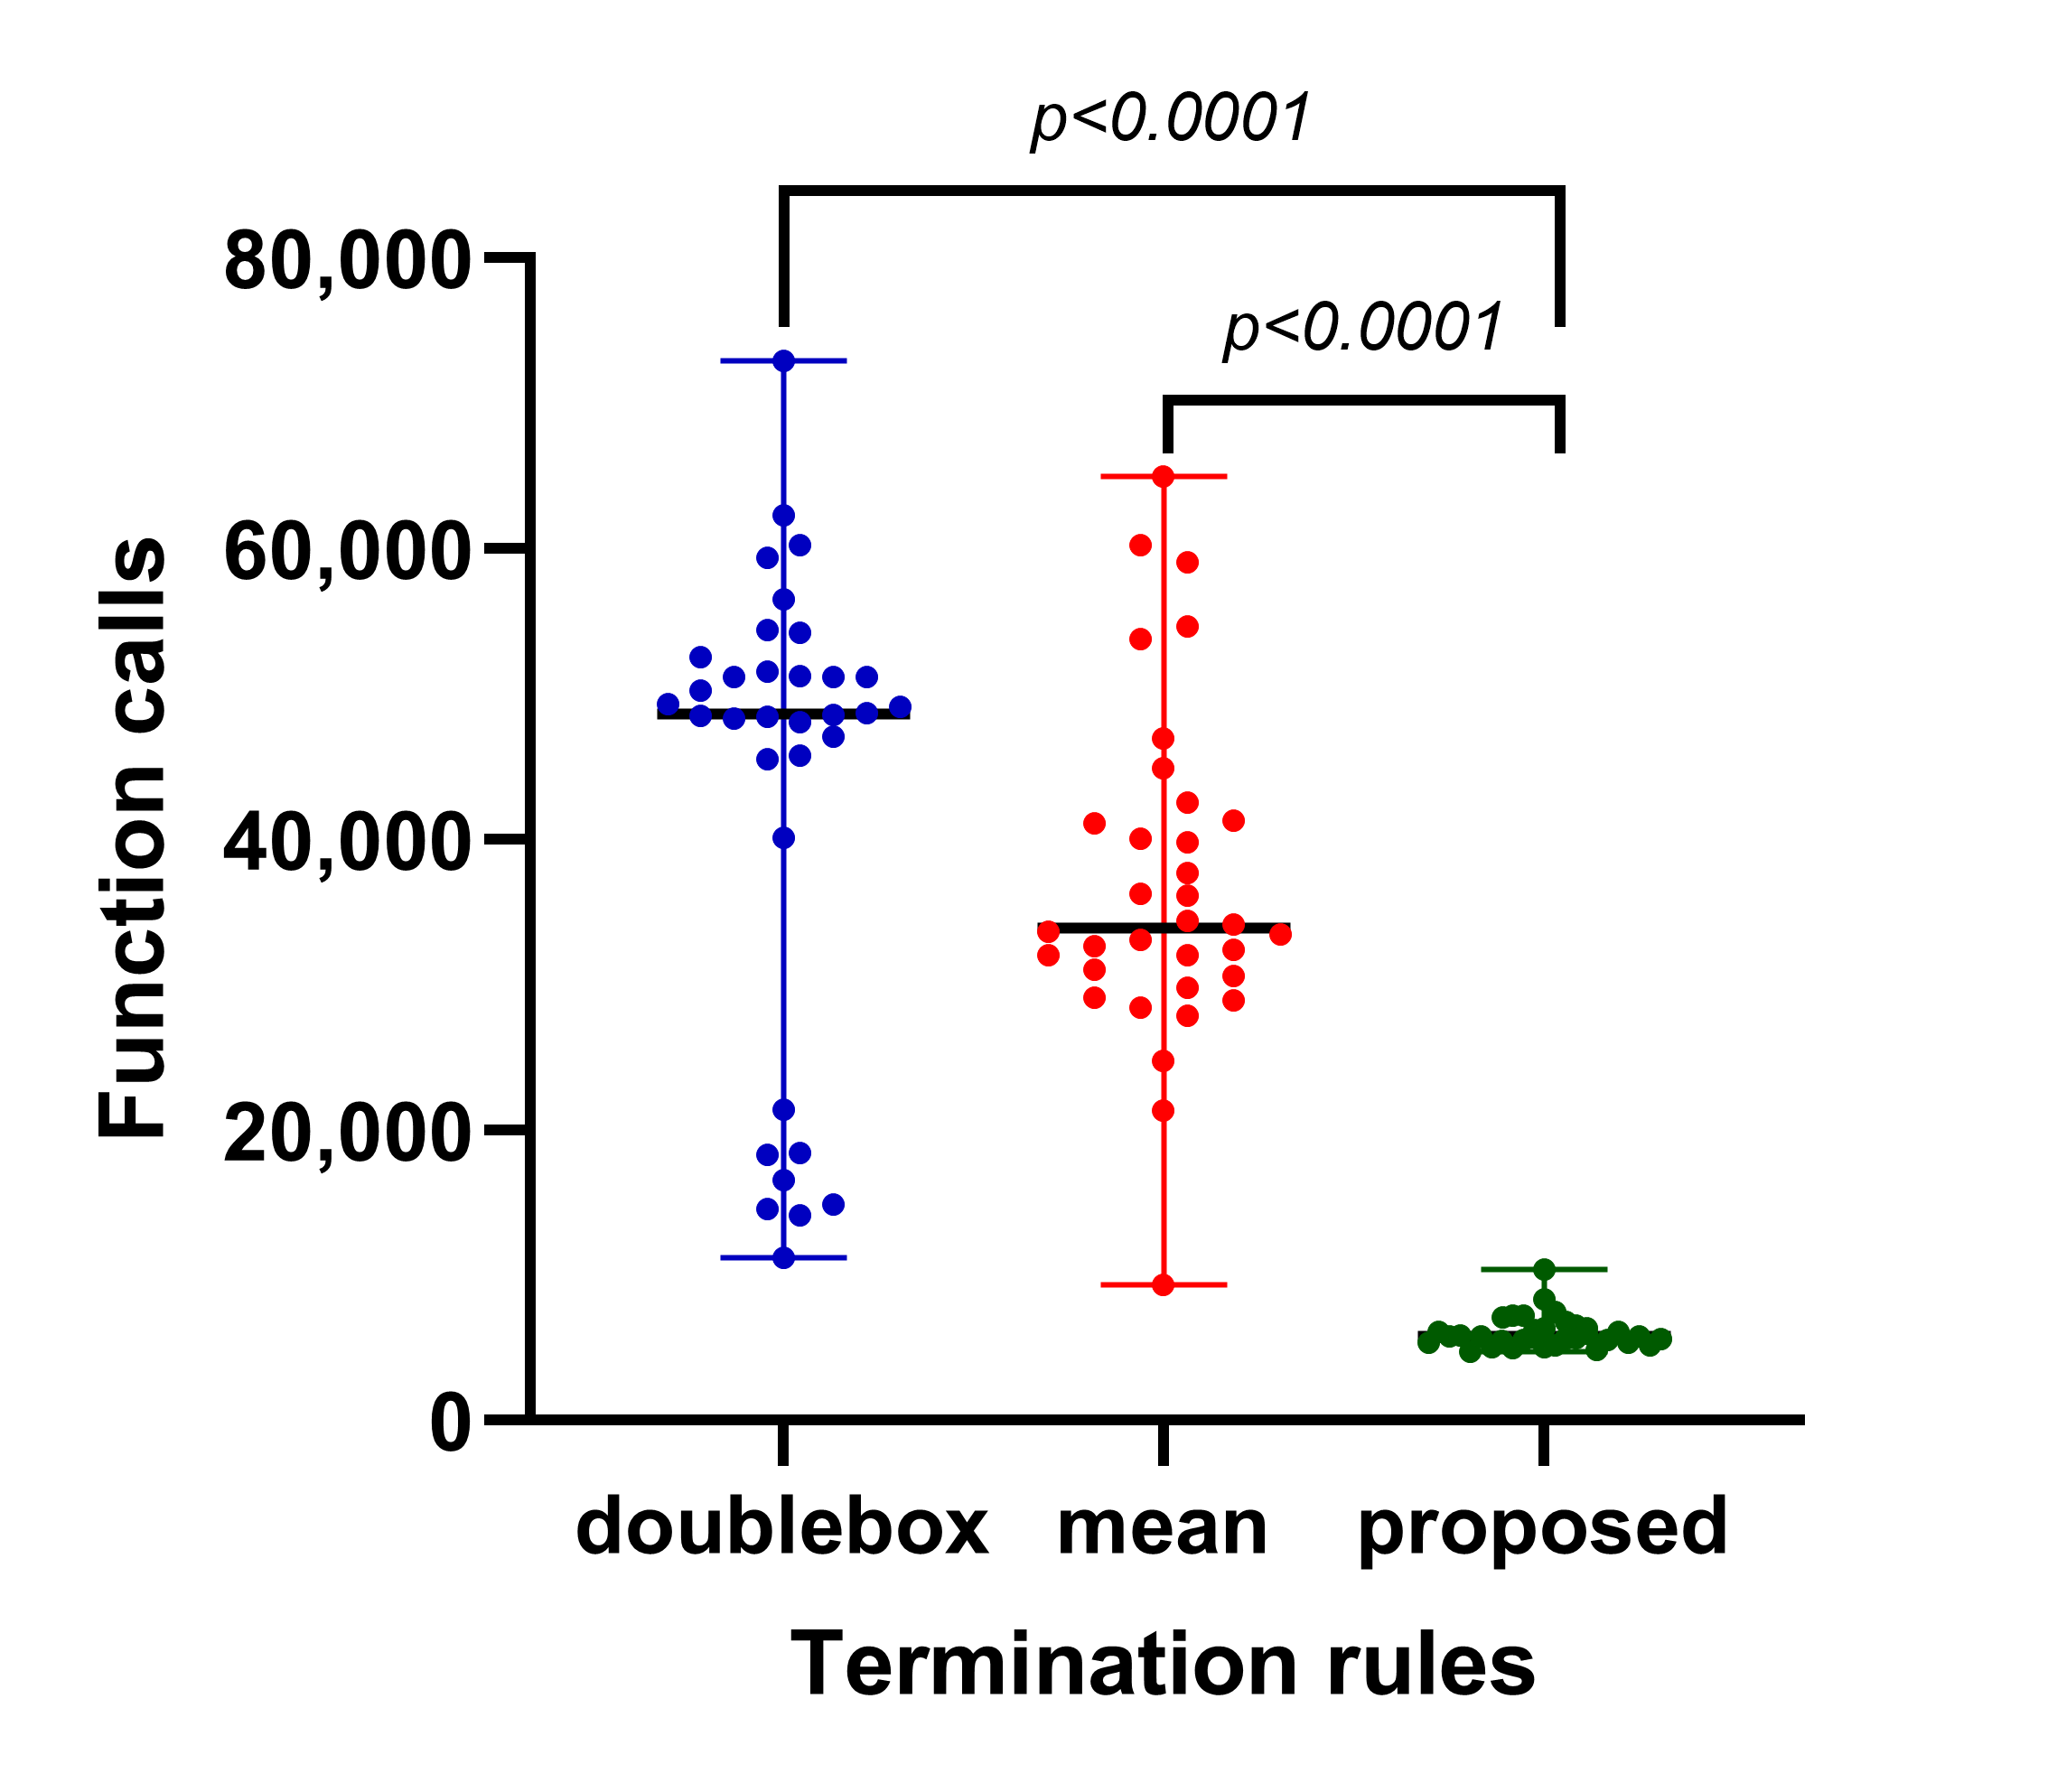
\includegraphics[scale=0.75]{wilcoxon}
\par\end{centering}
\caption{Wilcoxon rank-sum test results for the comparison of different termination
rules as used in the proposed parallel optimization technique and
for 5 processing units.\label{fig:Wilcoxon-rank-sum-test}}

\end{figure}
 A p-value of less than 0.05 (two-tailed) was used to determine statistical
significance and is indicated in bold.

An additional experiment was performed to assess the capabilities
of the parallel technique using the CM function for various values
of the dimension. This function is defined as:
\[
f(x)=\sum_{i=1}^{n}x_{i}^{2}-\frac{1}{10}\sum_{i=1}^{n}\cos\left(5\pi x_{i}\right)
\]
The proposed method was tested on this function for different values
of the dimension $n$ and for a variety of processing units and the
results are graphically illustrated in Figure \ref{fig:cmExper}.
\begin{figure}[H]
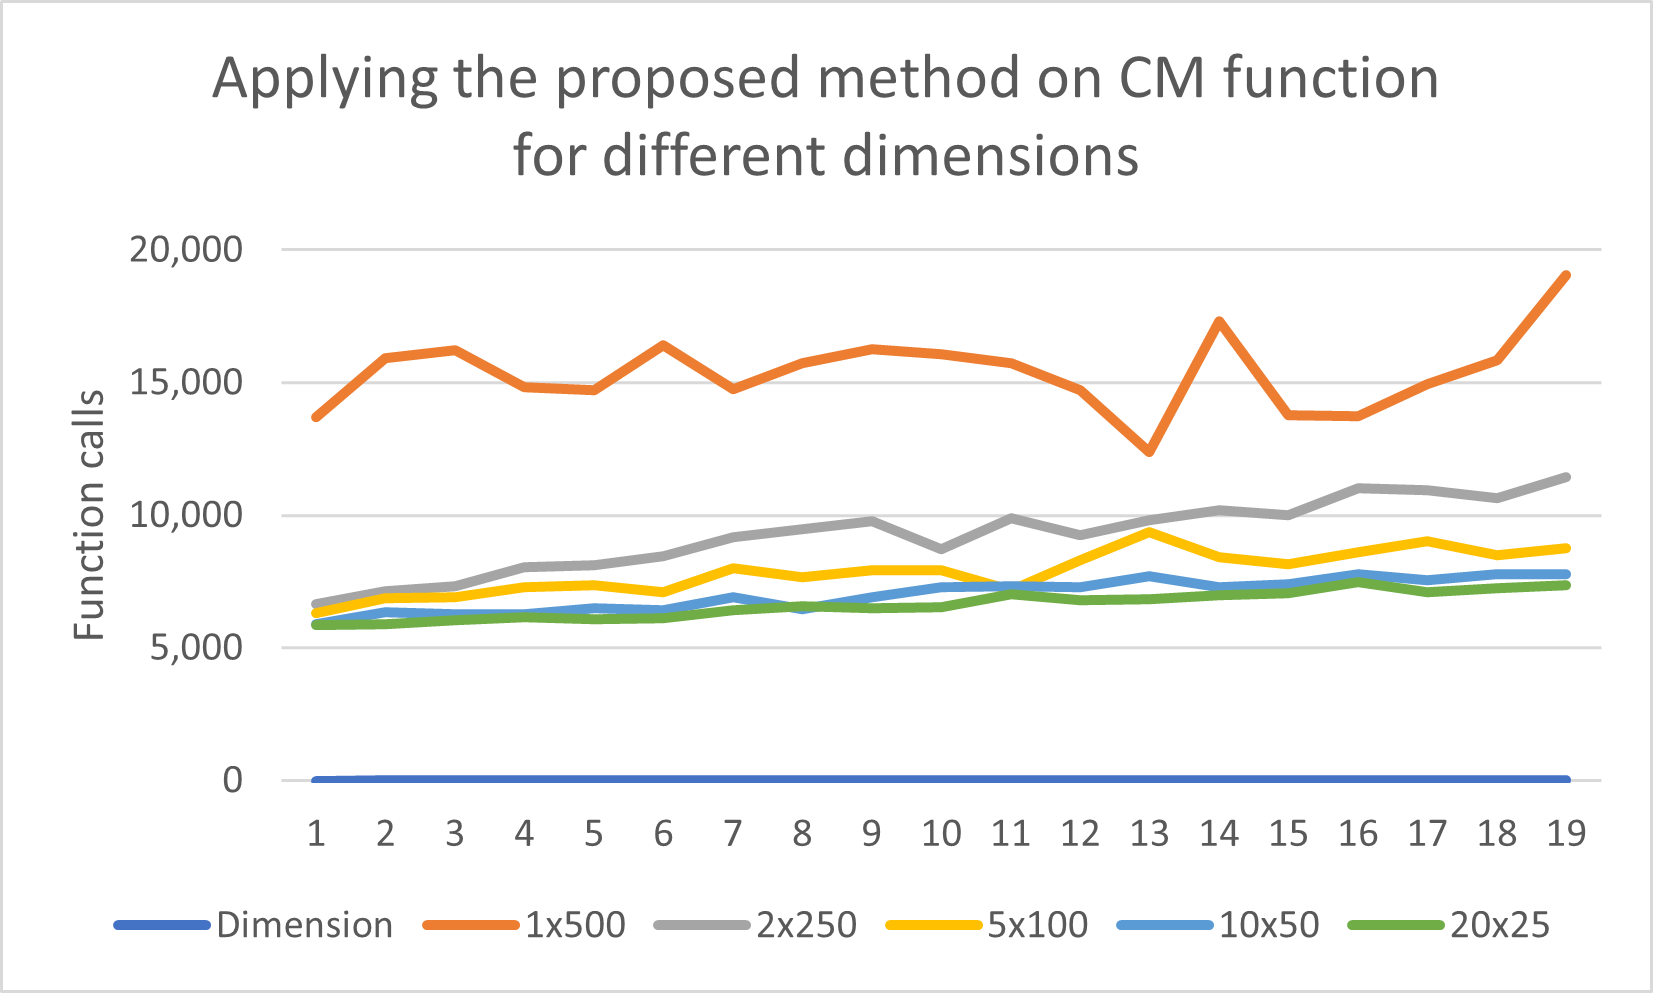
\includegraphics{cm}

\caption{Experiments using the proposed paralell technique and the CM function.
The dimension of the function $n$ varies from 1 to 20 and the number
of processing units changes from 1 to 20.\label{fig:cmExper}}

\end{figure}
From the experimental results it is obvious that the required number
of function calls is drastically reduced with the increase of computing
units from 1 to 2 or to 5. 

Also, the proposed method was applied on the GKLS function for different
versions of the function. The dimension of the function was in the
range $[2..5]$. In each dimension, 10 different versions of the functions
were used and average execution times and function calls were recorded.
Also, the proposed method was applied on the GKLS function using different
number of processing units. The average function calls from this experiment
are show graphically in Figure \ref{fig:experGklsCalls} and the average
execution times in Figure \ref{fig:gklsExperTime}.
\begin{figure}[H]
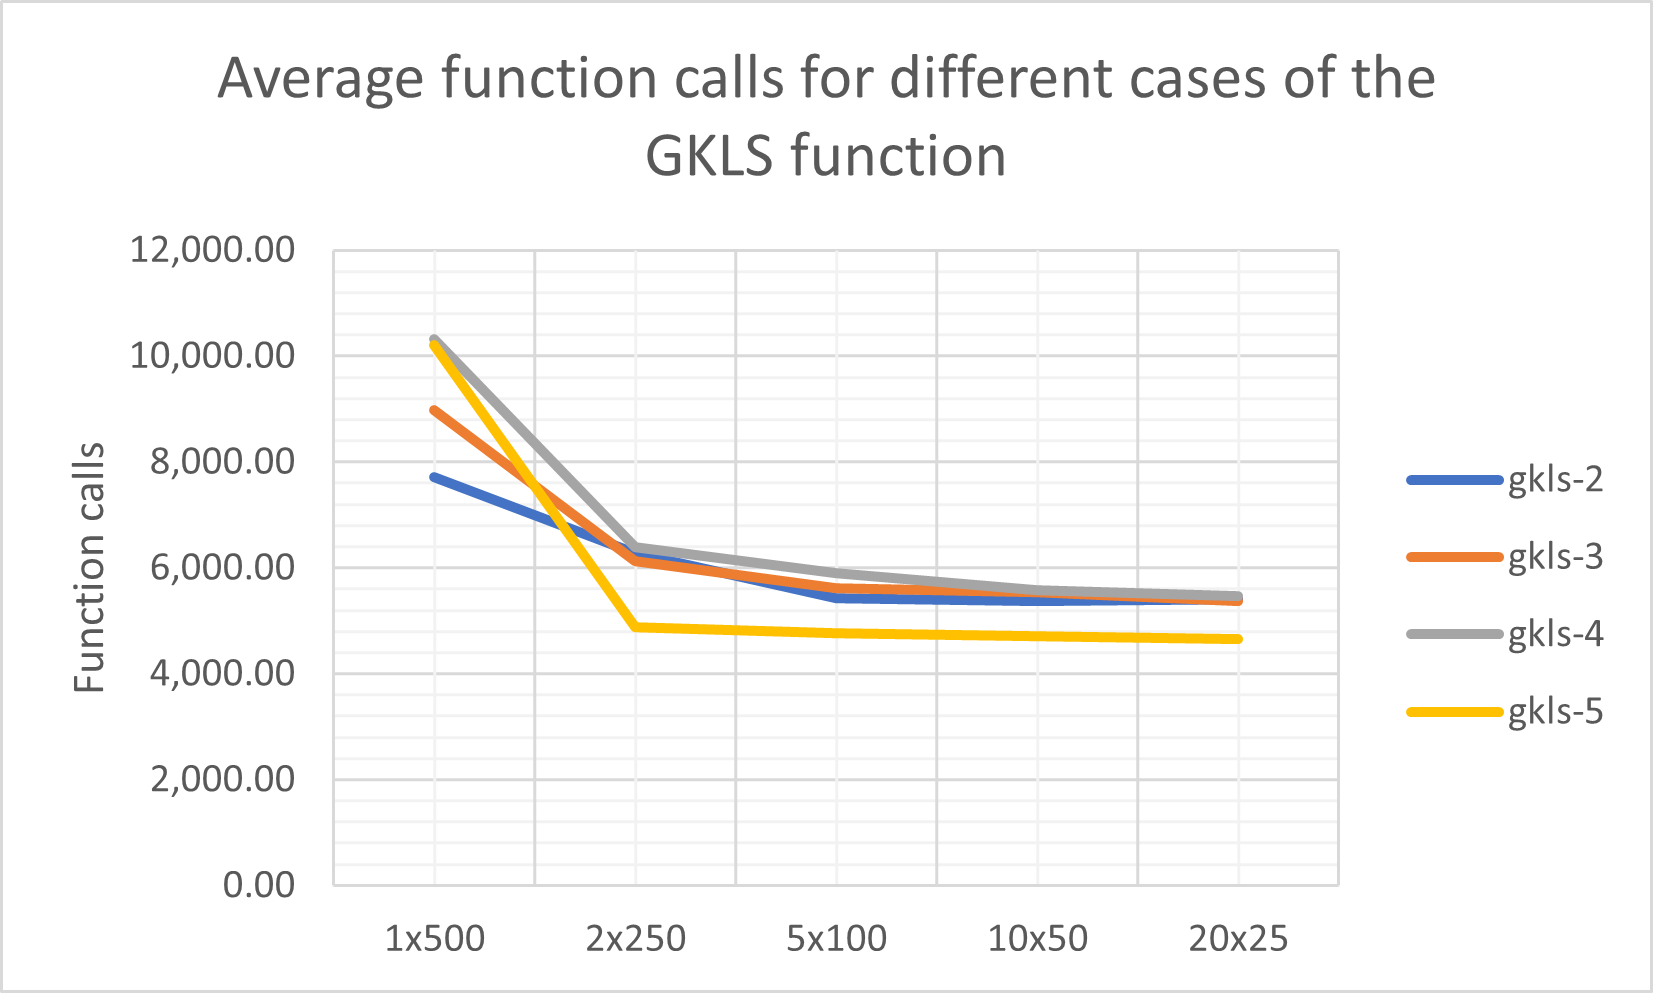
\includegraphics{gkls_calls}

\caption{Average function calls for the proposed method and different dimensions
of the GKLS function.\label{fig:experGklsCalls}}
\end{figure}
\begin{figure}[H]
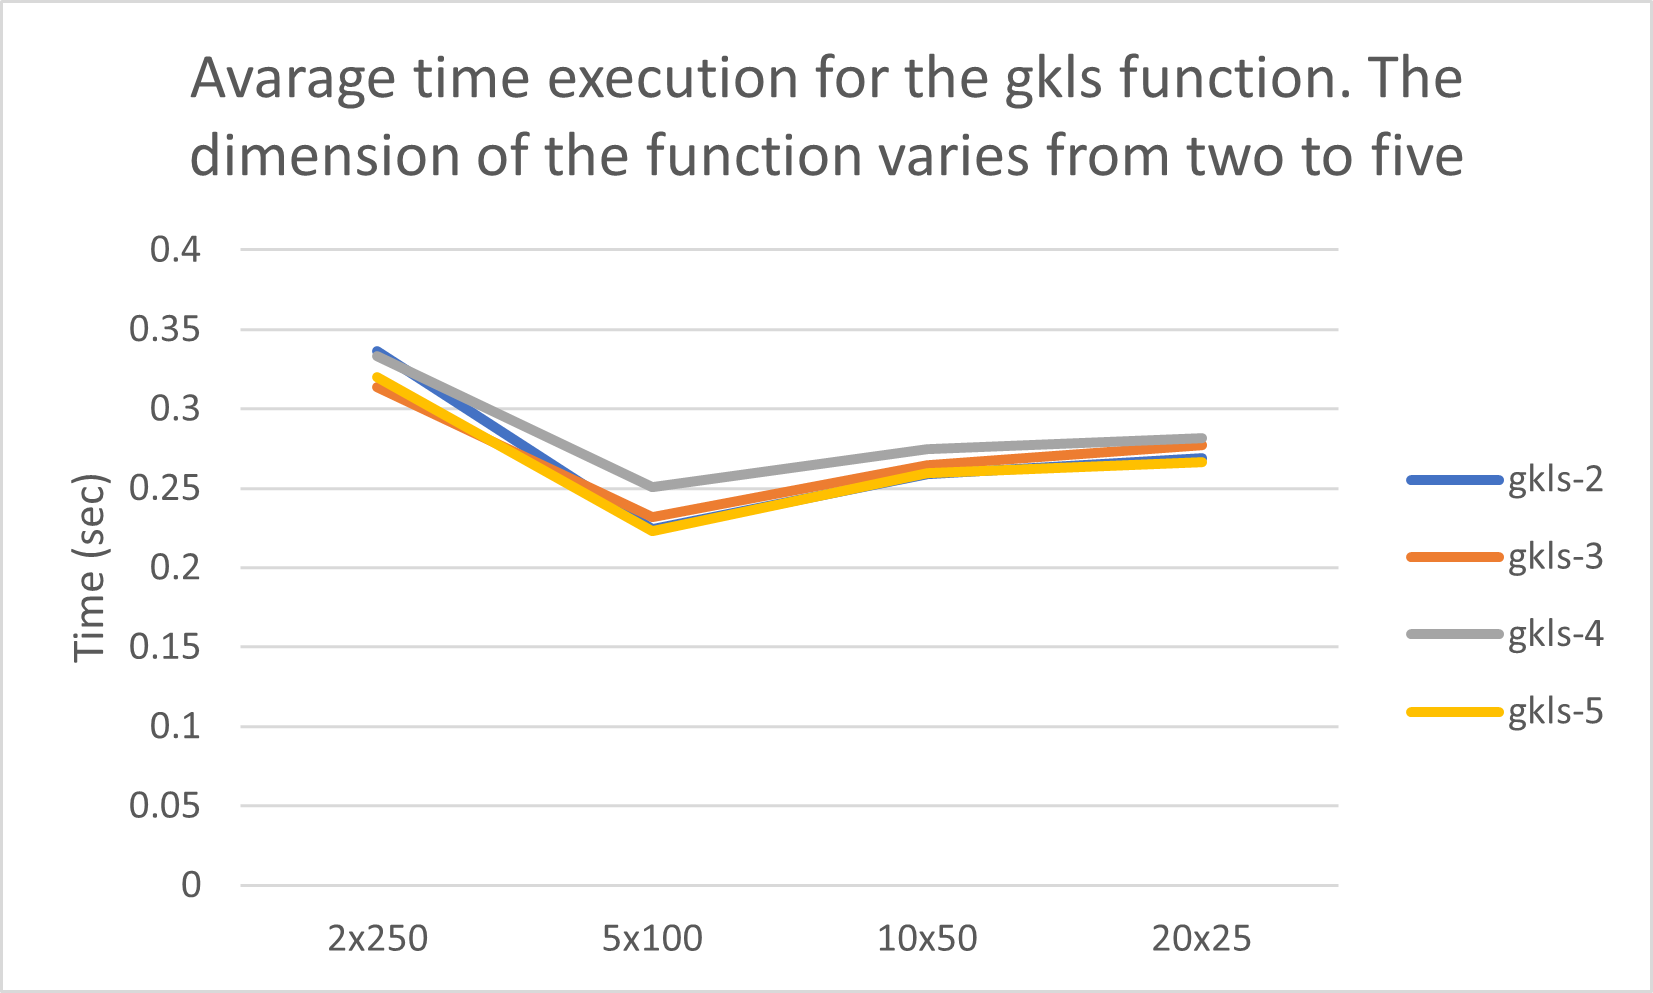
\includegraphics{gkls_time}

\caption{Average execution time for the GKLS function and the proposed method.
\label{fig:gklsExperTime}}
\end{figure}
 The graphs above show once again that adding processing units to
the proposed technique can reduce not only the execution time, as
expected, but also the required number of function calls. Furthermore,
in Figure \ref{fig:Speedup}, the behavior of speedup and efficiency
is depicted as a function of the number of computational units. It
is observed that speedup increases with the addition of more computational
units, while efficiency is initially high but gradually decreases.
\ref{fig:Speedup}.

\begin{figure}[H]
\begin{centering}
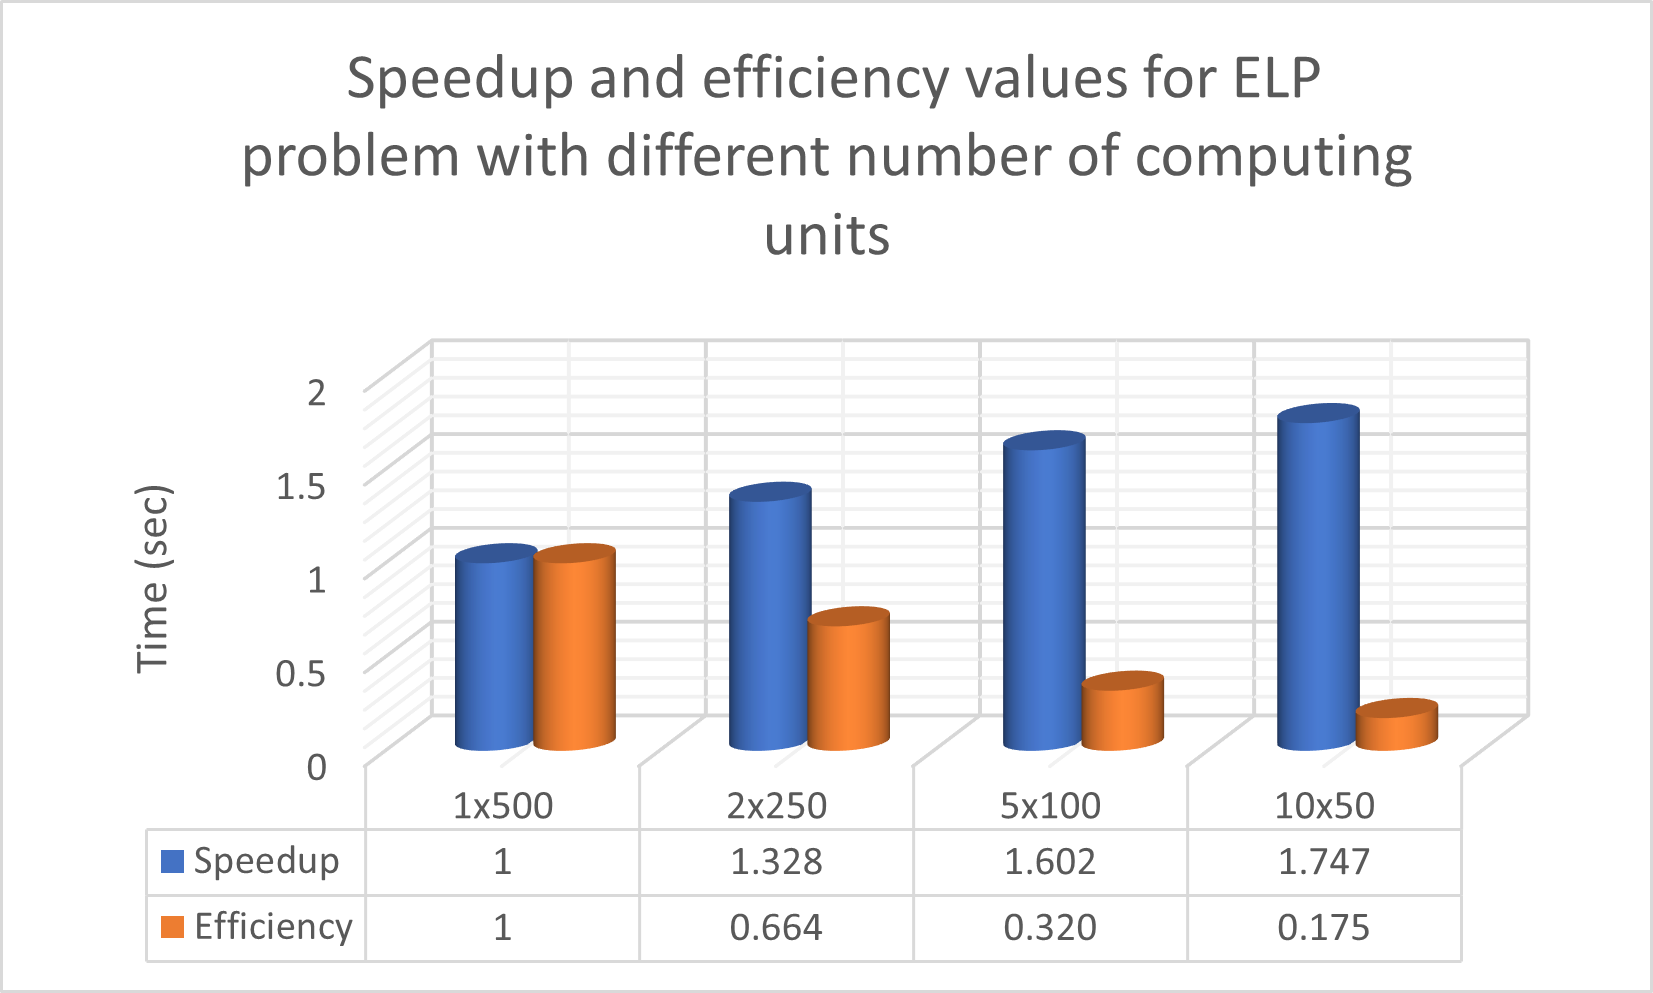
\includegraphics[scale=0.75]{speedup}
\par\end{centering}
\caption{Speedup and efficiency of the parallel approach.\label{fig:Speedup}}

\end{figure}


\section{Conclusions \label{sec:Conclusions}}

In this paper, the use of mixed termination rules for global optimization
methods was thoroughly presented, and a new global optimization method
that takes full advantage of parallel computing structures was afterward
proposed. The use of mixed termination rules leads a series of computational
global optimization techniques to find the global minimum of the objective
function faster, as was also shown by the experimental results. The
termination rules exploited are based on asymptotic criteria and are
general enough to be applicable to any global optimization problem
and stochastic global optimization technique.

Furthermore, the new stopping rule was utilized in a novel stochastic
global optimization technique that involves some basic global optimization
techniques. This method is designed to be executed in parallel computation
environments. At each step of the method, a different global optimization
method is also executed on each parallel computing unit, and these
different techniques exchange optimal solutions with each other. In
current work, the global optimization techniques of Differential Evolution,
Multistart and PSO were used in the processing units, but the method
can be generalized to use other stochastic optimization techniques,
such as genetic algorithms or simulated annealing. Also, the overall
method terminates with the combined termination rule proposed here,
and the experimental results performed on a series of well - known
test problems from the relevant literature seem to be very promising.

However, the present work is limited to a specific set of optimization
methods and termination criteria. Therefore, future extensions of
this work may include the integration of additional and more advanced
termination criteria, as well as the implementation of alternative
global optimization methods in the processing units, such as genetic
algorithms or variations of simulated annealing.

\vspace{6pt}

$ $

\authorcontributions{V.C., I.G.T and A.M.G conceived the idea and methodology and supervised
the technical part regarding the software. V.C. conducted the experiments.
A.M.G. performed the statistical analysis. I.G.T. and all other authors
prepared the manuscript. All authors have read and agreed to the published
version of the manuscript.}

\institutionalreview{Not applicable.}

\informedconsent{Not applicable.}

\dataavailability{Not applicable.}

\acknowledgments{This research has been financed by the European Union : Next Generation
EU through the Program Greece 2.0 National Recovery and Resilience
Plan , under the call RESEARCH -- CREATE -- INNOVATE, project name
“iCREW: Intelligent small craft simulator for advanced crew training
using Virtual Reality techniques\textquotedbl{} (project code:TAEDK-06195).}

\conflictsofinterest{The authors have no conflicts of interest to declare.}

\appendixtitles{no}

\appendixstart{}

\appendix

\begin{adjustwidth}{-\extralength}{0cm}{}


\reftitle{References}
\begin{thebibliography}{99}
\bibitem{go_physics1}M. Honda, Application of genetic algorithms
to modelings of fusion plasma physics, Computer Physics Communications
\textbf{231}, pp. 94-106, 2018.

\bibitem{go_physics2}X.L. Luo, J. Feng, H.H. Zhang, A genetic algorithm
for astroparticle physics studies, Computer Physics Communications
\textbf{250}, 106818, 2020.

\bibitem{go_physics3}T.M. Aljohani, A.F. Ebrahim, O. Mohammed, Single
and Multiobjective Optimal Reactive Power Dispatch Based on Hybrid
Artificial Physics--Particle Swarm Optimization, Energies \textbf{12},
2333, 2019.

\bibitem{go_chemistry1}P.M. Pardalos, D. Shalloway, G. Xue, Optimization
methods for computing global minima of nonconvex potential energy
functions, Journal of Global Optimization \textbf{4}, pp. 117-133,
1994.

\bibitem{go_chemistry2}A. Liwo, J. Lee, D.R. Ripoll, J. Pillardy,
H. A. Scheraga, Protein structure prediction by global optimization
of a potential energy function, Biophysics \textbf{96}, pp. 5482-5485,
1999.

\bibitem{go_chemistry3}J. An, G.He, F. Qin, R. Li, Z. Huang, A new
framework of global sensitivity analysis for the chemical kinetic
model using PSO-BPNN, Computers \& Chemical Engineering \textbf{112},
pp. 154-164, 2018.

\bibitem{go_econ1}Zwe-Lee Gaing, Particle swarm optimization to solving
the economic dispatch considering the generator constraints, IEEE
Transactions on \textbf{18} Power Systems, pp. 1187-1195, 2003.

\bibitem{go_econ2}M. Basu, A simulated annealing-based goal-attainment
method for economic emission load dispatch of fixed head hydrothermal
power systems, International Journal of Electrical Power \& Energy
Systems \textbf{27}, pp. 147-153, 2005.

\bibitem{go_med1}Y. Cherruault, Global optimization in biology and
medicine, Mathematical and Computer Modelling \textbf{20}, pp. 119-132,
1994.

\bibitem{go_med2}Eva K. Lee, Large-Scale Optimization-Based Classification
Models in Medicine and Biology, Annals of Biomedical Engineering \textbf{35},
pp 1095-1109, 2007.

\bibitem{interval1}M.A. Wolfe, Interval methods for global optimization,
Applied Mathematics and Computation \textbf{75}, pp. 179-206, 1996.

\bibitem{interval2}T. Csendes and D. Ratz, Subdivision Direction
Selection in Interval Methods for Global Optimization, SIAM J. Numer.
Anal. \textbf{34}, pp. 922--938, 1997. 

\bibitem{Kawachi} Kawachi, M., Ando, N. ( 1989). Genetic Algorithms
in Search, Optimization \& Machine Learning. Artificial Intelligence,
Vol.: 7, Issue: 1, pp.: 168. Doi: https://doi.org/10.11517/jjsai.7.1\_168 

\bibitem{Kirkpatrick} Kirkpatrick, S., Gelatt, C.D., Vecchi, M.P.
(1983). Optimization by simulated annealing. Science, Vol. 220, Issue:
4598, pp.: 671--680. DOI: 10.1126/science.220.4598.671 {[}CrossRef{]}
{[}PubMed{]}

\bibitem{Hashim} Hashim, F.A., Houssein, E.H., Mabrouk, M.S., Al-Atabany,W.,
Mirjalili, S. (2019). Henry gas solubility optimization: A novel physics
based algorithm. Future Generation Computer Systems: Vol.: 101, pp.:
646--667. Doi: https: 10.1016/j.future.2019.07.015

\bibitem{Rashedi} Rashedi, E., Nezamabadi-Pour, H., Saryazdi, S.
(2009). GSA: A gravitational search algorithm. Information Sciences:
Vol.: 179, pp.:2232--2248. https://doi.org/10.1016/j.ins.2009.03.004

\bibitem{Du-Wu} Du, H., Wu, X., Zhuang, J. (2006). Small-World Optimization
Algorithm for Function Optimization. In Proceedings of the International
Conference on Natural Computation, Xi’an, China, 24--28 September
2006, pp. 264--273. Doi: 10.1007/11881223\_33 

\bibitem{Goldberg} Goldberg, D.E., Holland, J.H. (1988). Genetic
Algorithms and Machine Learning. Machine Learning (3): pp.: 95--99.
Doi: 10.1023/A:1022602019183

\bibitem{Das} Das, S. , Suganthan, P.N. (2011). Differential evolution:
A survey of the state-of-the-art. IEEE Transactions on Evolutionary
Computation, Vol.: 15, Issue:1, pp.: 4--31. Doi: 10.1109/TEVC.2010.2059031

\bibitem{Charilogis} V. Charilogis , I.G. Tsoulos, A. Tzallas, E.
Karvounis, Modifications for the Differential Evolution Algorithm,
Symmetry \textbf{14}, 447, 2022.

\bibitem{Kennedy} Kennedy, J., Eberhart, R. (1995). Particle Swarm
Optimization. In Proceedings of the ICNN’95---International Conference
on Neural Networks, Perth,WA, Australia, 27 November--1 December
1995, Vol.: 4, pp. 1942--1948. Doi: 10.1109/ICNN.1995.488968

\bibitem{Charilogis2} V. Charilogis, I.G. Tsoulos, Toward an Ideal
Particle Swarm Optimizer for Multidimensional Functions, Information
\textbf{13}, 217, 2022.

\bibitem{Dorigo} Dorigo, M., Maniezzo, V., Colorni, A. (1996). Ant
system: Optimization by a colony of cooperating agents. IEEE Transactions
on Systems, Man, and Cybernetics, Part B (Cybernetics), Vol.: 26,
pp.: 29--41. Doi: 10.1109/3477.484436 

\bibitem{Yang} Yang, X.S., Gandomi, A.H. (2012). Bat algorithm: A
novel approach for global engineering optimization. Engineering Computations,
Vol.: 29, pp.: 464--483. Doi: https://doi.org/10.1108/02644401211235834

\bibitem{Mirjalili} Mirjalili, S., Lewis, A. (2016). The whale optimization
algorithm. Advances in Engineering Softwar, Vol.: 95, pp.: 51--67.
Doi: https://doi.org/10.1016/j.advengsoft.2016.01.008

\bibitem{Saremi} Saremi, S., Mirjalili, S., Lewis, A. (2017). Grasshopper
optimisation algorithm: Theory and application. Advances in Engineering
Software, Vol.: 105, pp.: 30--47.Doi: https://doi.org/10.1016/j.advengsoft.2017.01.004.

\bibitem{Rao} Rao, R.V., Savsani, V.J., Vakharia, D. (2011). Teaching--learning-based
optimization: A novel method for constrained mechanical design optimization
problems. Computer-Aided Design, Vol.: 43, pp.: 303--315. Doi: https://doi.org/10.1016/j.cad.2010.12.015

\bibitem{parallel-pso}J. F. Schutte, J. A. Reinbolt, B. J. Fregly, R.
T. Haftka, A. D. George, Parallel global optimization with the particle
swarm algorithm, International journal for Numerical methods in Engineering
\textbf{61}, pp. 2296-2315, 2004.

\bibitem{parallel-multistart}J. Larson and S.M. Wild, Asynchronously
parallel optimization solver for finding multiple minima, Mathematical
Programming Computation \textbf{10}, pp. 303-332, 2018.

\bibitem{parallel-doublepop}I.G. Tsoulos, A. Tzallas, D. Tsalikakis,
PDoublePop: An implementation of parallel genetic algorithm for function
optimization, Computer Physics Communications \textbf{209}, pp. 183-189,
2016.

\bibitem{msgpu1}R. Kamil, S. Reiji, An Efficient GPU Implementation
of a Multi-Start TSP Solver for Large Problem Instances, Proceedings
of the 14th Annual Conference Companion on Genetic and Evolutionary
Computation, pp. 1441-1442, 2012.

\bibitem{msgpu2}Van Luong T., Melab N., Talbi EG. (2011) GPU-Based
Multi-start Local Search Algorithms. In: Coello C.A.C. (eds) Learning
and Intelligent Optimization. LION 2011. Lecture Notes in Computer
Science, vol 6683. Springer, Berlin, Heidelberg. https://doi.org/10.1007/978-3-642-25566-3\_24

\bibitem{msgpu3}K. Barkalov, V. Gergel, Parallel global optimization
on GPU, J Glob Optim \textbf{66}, pp. 3--20, 2016. 

\bibitem{Low Gon} Low, Y., Gonzalez, J., Kyrola, A., Bickson,D.,
Guestrin, C., Hellerstein, J. (2010). GraphLab: A New Framework For
Parallel Machine Learning. Source: arXiv, Computer Science. 

\bibitem{Yangyang} Yangyang, L., Liu, G., Lu, G., Jiao, L., Marturi,
N. \& Shang, R. (2019). Hyper-Parameter Optimization Using MARS Surrogate
for Machine-Learning Algorithms. IEEE Transactions on Emerging Topics
in Computational Intelligence, pp(99):1-11. DOI: 10.1109/TETCI.2019.2918509. 

\bibitem{Yamashiro}Yamashiro, H. \& Nonaka, H. (2021). Estimation
of processing time using machine learning and real factory data for
optimization of parallel machine scheduling problem. ScienceDirect:
Operations Research Perspectives, Vol.:8, 2021, Doi: https://doi.org/10.1016/j.orp.2021.100196
.

\bibitem{Kim Tsai} Kim, H.S. \& Tsai, L. (2003). Design Optimization
of a Cartesian Parallel Manipulator. Journal of Mechanical Design,125(1):43-51.
Doi: https://doi.org/10.1115/1.1543977 .

\bibitem{Oh Jong} Oh, S., Jong Jang,H. \& Pedrycz, W. (2009). The
design of a fuzzy cascade controller for ball and beam system: A study
in optimization with the use of parallel genetic algorithms. ScienceDirect:
Engineering Applications of Artificial Intelligence, 22(2):261-271.
Doi: https://doi.org/10.1016/j.engappai.2008.07.003 .

\bibitem{Fatehi} Fatehi, M., Toloei, A., Zio, E., Niaki, S.T.A. \&
Kesh,B. (2023). Robust optimization of the design of monopropellant
propulsion control systems using an advanced teaching-learning-based
optimization method. ScienceDirect: Engineering Applications of Artificial
Intelligence, Vol.:126, Part: A. 

\bibitem{Cai Yang} Cai, J., Yang, H., Lai, T. \& Xu, K.(2023). Parallel
pump and chiller system optimization method for minimizing energy
consumption based on a novel multi-objective gorilla troops optimizer.
ScienceDirect: Journal Of Building Engineering, Vol.: 76, Doi: https://doi.org/10.1016/j.jobe.2023.107366

\bibitem{Yu Shahabi} Yu, Y. \& Shahabi, L. (2023). Engineering Application
of Artificial Intelligence: Optimal infrastructure in microgrids with
diverse uncertainties based on demand response, renewable energy sources
and two-stage parallel optimization algorithm. ScienceDirect. Vol.:123,
Part b. Doi: https://doi.org/10.1016/j.engappai.2023.106233 

\bibitem{Ramirez} Ramirez-Gil, F.J., Pere-Madrid, C.M., Nelli Silva,
E.C. \& Montealerge-Rubio, W. (2021). Sustainable Computing: Informatics
and Systems: Parallel computing for the topology optimization method:
Performance metrics and energy consumption analysis in multiphysics
problems. Vol.:30, Doi: https://doi.org/10.1016/j.suscom.2020.100481 

\bibitem{Tavakolan} Tavakolan, M., Mostafazadeh, F., Eirdmousa, S.J.,
Safari, A. \& Mirzai, K. (2022). A parallel computing simulation-based
multi-objective optimization framework for economic analysis of building
energy retrofit: A case study in Iran. ScienceDirect: Journal of Building
Engineering, Vol.: 45, Doi: https://doi.org/10.1016/j.jobe.2021.103485

\bibitem{Lin} Lin, G. (2020). Parallel optimization n based operational
planning to enhance the resilience of large-scale power systems. Mississippi
State University, Scholars Junction. Online: https://scholarsjunction.msstate.edu/cgi/viewcontent.cgi?article=4435\&context=td

\bibitem{Pang} Pang, M. \& Shoemaker, C.A. (2023). Comparison of
parallel optimization algorithms on computationally expensive groundwater
remediation designs. Sience of the Total Environment: 857(3), Doi:
https://doi.org/10.1016/j.scitotenv.2022.159544

\bibitem{Ezugwu} Ezugwu, A. (2023). A general Framework for Utilizing
Metaheuristic Optimization for Sustainable Unrelated Parallel Machine
Scheduling: A concise overview. Arxiv, Computer Science, Neural and
Evolutionary Computing. Doi: https://doi.org/10.48550/arXiv.2311.12802 

\bibitem{Censor} Censor, Y. \& Zenios, S. (1997). Parallel Optimization:
Theory, Algorithms and Applications. Publisher: Oxford University
Press, USAISBN: ISBN-13: 978-0195100624. DOI: 10.1093/oso/9780195100624.001.0001 

\bibitem{go_par1}E. Onbaşoğlu, L. Özdamar, Parallel simulated annealing
algorithms in global optimization. Journal of global optimization
\textbf{19}, pp. 27-50, 2001.

\bibitem{go_par2}J.F. Schutte, J.A. Reinbolt, B.J. Fregly, R.T. Haftka,
A.D. George, Parallel global optimization with the particle swarm
algorithm. International journal for numerical methods in engineering
\textbf{61}, pp. 2296-2315, 2004.

\bibitem{go_par3}Regis, R. G., \& Shoemaker, C. A. (2009). Parallel
stochastic global optimization using radial basis functions. INFORMS
Journal on Computing, 21(3), 411-426.

\bibitem{pga_survey1}R. Shonkwiler, Parallel genetic algorithms.
In ICGA (pp. 199-205), 1993.

\bibitem{pga_survey2}E. Cantú-Paz, A survey of parallel genetic algorithms,
Calculateurs paralleles, reseaux et systems repartis \textbf{10},
pp. 141-171, 1998.

\bibitem{go_add_par1}Rudy Alex Gallegos Lizárraga (2024). Parallel
Computing for Real-Time Image Processing. DOI:10.20944/preprints202408.0040.v1 

\bibitem{go_add_par2}Asif Afzal, Zahid Ansari, Ahmed Rimaz Faizabadi
\& M. K. Ramis (2017).Parallelization Strategies for Computational
Fluid Dynamics Software: State of the Art Review. Archives of Computational
Methods in Engineering. Volume 24, pages 337--363, (2017).

\bibitem{go_add_par3}You Zou, Yuejie Zhu, Yaohang Li, Fang-Xiang
Wu, Jianxin Wang (2021).Parallel computing for genome sequence processing.
DOI: 10.1093/bib/bbab070 

\bibitem{go_add_par4}C.B. Lucasius, G. Kateman (1991).Genetic algorithms
for large-scale optimization in chemometrics: An application. TrAC
Trends in Analytical Chemistry. Volume 10, Issue 8, September 1991,
Pages 254-261. https://doi.org/10.1016/0165-9936(91)85132-B 

\bibitem{go_add_par5}Sangeetha M., Sabari A. (2018). Genetic optimization
of hybrid clustering algorithm in mobile wireless sensor networks.
Sensor Review:Volume 38 Issue 4.

\bibitem{go_add_par6}Ali Ghaheri, Saeed Shoar, Mohammad Naderan \&
Sayed Shahabuddin Hoseini (2015).The Applications of Genetic Algorithms
in Medicine. Journal List Oman Med J. Nov; 30(6): 406--416. doi:
10.5001/omj.2015.82 

\bibitem{Marini} Marini, F. \& Walczak, B. (2015). Particle swarm
optimization (PSO). A tutorial. Chemometrics and Intelligent Laboratory
Systems. Volume 149, Part B, p.:153-165. Doi: https://doi.org/10.1016/j.chemolab.2015.08.020

\bibitem{Garc=0000EDa-Gonzalo} García-Gonzalo, E. \& Fernández-Martínez,
J. L. (2012). A Brief Historical Review of Particle Swarm Optimization
(PSO). Journal of Bioinformatics and Intelligent Control, Volume 1,
Number 1, June 2012, pp. 3-16(14). American Scientific Publishers.
DOI:https://doi.org/10.1166/jbic.2012.1002 

\bibitem{Jain} Jain, M., Saihjpal, V., Singh, N. \& Singh, S.B. (2022).
An Overview of Variants and Advancements of PSO Algorithm. MDPI, Applied
Sciences: 12, 8392. Doi:https://doi.org/10.3390/ app12178392 . 

\bibitem{psophysics1}Anderson Alvarenga de Moura Meneses, Marcelo
Dornellas, Machado Roberto Schirru, Particle Swarm Optimization applied
to the nuclear reload problem of a Pressurized Water Reactor, Progress
in Nuclear Energy \textbf{51}, pp. 319-326, 2009.

\bibitem{psophysics2}Ranjit Shaw, Shalivahan Srivastava, Particle
swarm optimization: A new tool to invert geophysical data, Geophysics
\textbf{72}, 2007.

\bibitem{psochem1}C. O. Ourique, E.C. Biscaia, J.C. Pinto, The use
of particle swarm optimization for dynamical analysis in chemical
processes, Computers \& Chemical Engineering \textbf{26}, pp. 1783-1793,
2002.

\bibitem{psochem2}H. Fang, J. Zhou, Z. Wang et al, Hybrid method
integrating machine learning and particle swarm optimization for smart
chemical process operations, Front. Chem. Sci. Eng. \textbf{16}, pp.
274--287, 2022.

\bibitem{psomed1}M.P. Wachowiak, R. Smolikova, Yufeng Zheng, J.M.
Zurada, A.S. Elmaghraby, An approach to multimodal biomedical image
registration utilizing particle swarm optimization, IEEE Transactions
on Evolutionary Computation \textbf{8}, pp. 289-301, 2004.

\bibitem{psomed2}Yannis Marinakis. Magdalene Marinaki, Georgios Dounias,
Particle swarm optimization for pap-smear diagnosis, Expert Systems
with Applications \textbf{35}, pp. 1645-1656, 2008. 

\bibitem{psoecon}Jong-Bae Park, Yun-Won Jeong, Joong-Rin Shin, Kwang
Y. Lee, An Improved Particle Swarm Optimization for Nonconvex Economic
Dispatch Problems, IEEE Transactions on Power Systems \textbf{25},
pp. 156-16\textbf{216}6, 2010.

\bibitem{Feoktistov} Feoktistov, V. (2006). Differential Evolution.
In Search of Solutions. Optimization and Its Appl;ications, Springer.
Doi: https://doi.org/10.1007/978-0-387-36896-2 

\bibitem{Bilal} Bilal, M.P., Zaheer, H., Garcia-Hernandez, L. \&
Abraham, A. (2020). Differential Evolution: A review of more than
two decades of research. Engineering Applications of Artificial Intelligence
90 (2020) 103479. Doi: https://doi.org/10.1016/j.engappai.2020.103479 

\bibitem{de_app1}P. Rocca, G. Oliveri, A. Massa, Differential Evolution
as Applied to Electromagnetics, IEEE Antennas and Propagation Magazine.
\textbf{53}, pp. 38-49, 2011.

\bibitem{de_app2}W.S. Lee, Y.T. Chen, Y. Kao, Optimal chiller loading
by differential evolution algorithm for reducing energy consumption,
Energy and Buildings \textbf{43}, pp. 599-604, 2011.

\bibitem{de_app3}Y. Yuan, H. Xu, Flexible job shop scheduling using
hybrid differential evolution algorithms, Computers \& Industrial
Engineering \textbf{65}, pp. 246-260, 2013.

\bibitem{de_app4}L. Xu, H. Jia, C. Lang, X. Peng, K. Sun, A Novel
Method for Multilevel Color Image Segmentation Based on Dragonfly
Algorithm and Differential Evolution, IEEE Access \textbf{7}, pp.
19502-19538, 2019.

\bibitem{Marti} Marti, R., Resende, M.G.C. \& Ribeiro, C. (2013).
Multi-start methods for combinatorial optimization. European Journal
of Operational Research Volume 226, Issue 1, 1 April 2013, Pages 1-8.
Doi: https://doi.org/10.1016/j.ejor.2012.10.012 

\bibitem{Marti Moreno} Marti, R., Moreno-Vega, J. \& Duarte, A. (2010).
Advanced Multi-start Methods. Handbook of Metaheuristics, pp: 265--281.

\bibitem{Tu Mayne} Tu, W. \& Mayne, R.W. (2002). Studies of multi-start
clustering for global optimization. International Journal for Numerical
Methods in Engineering. Doi: https://doi.org/10.1002/nme.400. 

\bibitem{bfgs_main}Dai, Y. H. (2002). Convergence properties of the
BFGS algoritm. SIAM Journal on Optimization, 13(3), 693-701.

\bibitem{Tsoulos} Tsoulos, I.G. Modifications of real code genetic
algorithm for global optimization. Appl. Math. Comput. 2008, 203,
598--607.

\bibitem{Gaviano} M. Gaviano, D.E. Ksasov, D. Lera, Y.D. Sergeyev,
Software for generation of classes of test functions with known local
and global minima for global optimization, ACM Trans. Math. Softw.
\textbf{29}, pp. 469-480, 2003.

\bibitem{Lennard} J.E. Lennard-Jones, On the Determination of Molecular
Fields, Proc. R. Soc. Lond. A \textbf{ 106}, pp. 463--477, 1924.

\bibitem{Zabinsky} Z.B. Zabinsky, D.L. Graesser, M.E. Tuttle, G.I.
Kim, Global optimization of composite laminates using improving hit
and run, In: Recent advances in global optimization, pp. 343-368,
1992.

\bibitem{pde}Charilogis, V.; Tsoulos, I.G. A Parallel Implementation
of the Differential Evolution Method. Analytics 2023, 2, 17--30.

\bibitem{ppso}Charilogis, V.; Tsoulos, I.G.; Tzallas, A. (2023).
An Improved Parallel Particle Swarm Optimization. SN Computer Science
(2023) 4:766

\bibitem{Floudas} C.A. Floudas, P.M. Pardalos, C. Adjiman, W. Esposoto,
Z. G$\ddot{\mbox{u}}$m$\ddot{\mbox{u}}$s, S. Harding, J. Klepeis,
C. Meyer, C. Schweiger, Handbook of Test Problems in Local and Global
Optimization, Kluwer Academic Publishers, Dordrecht, 1999.

\bibitem{Montaz Ali}M. Montaz Ali, Charoenchai Khompatraporn, Zelda
B. Zabinsky, A Numerical Evaluation of Several Stochastic Algorithms
on Selected Continuous Global Optimization Test Problems, Journal
of Global Optimization \textbf{31}, pp 635-672, 2005.

\bibitem{Gao}Gao, Z.M., Zhao, J., Hu,Y.R., Chen, H.F. (2021).The
Challenge for the Nature - Inspired Global Optimization Algorithms:
Non-Symmetric Benchmark Functions. IEEE Access, July 26, 2021.

\bibitem{openMP} R. Chandra, L. Dagum, D. Kohr, D. Maydan,J. McDonald
and R. Menon, Parallel Programming in OpenMP, Morgan Kaufmann Publishers
Inc., 2001.

\bibitem{gwo}S. Mirjalili, S.M. Mirjalili, A. Lewis, Grey wolf optimizer.
Advances in engineering software \textbf{69}, pp. 46-61, 2014.

\end{thebibliography}

\end{adjustwidth}{}
\end{document}
